%!TEX root = paper.tex
%*****************************************************************************%
%		 			Results
%*****************************************************************************%
%===================================================================%
% 				Simulation results
%===================================================================%
\subsection{Results on synthetic functional connectome data}
\label{subsec:result,synth}
In order to evaluate the validity of our proposed method, we compared the performance of four linear classifiers trained on the synthetic functional connectome data described in Section~\ref{subsec:synthetic,4d,conn}, where the training set consists of $100$ samples with $50$ patients and $50$ controls.
Specifically, we solved the regularized ERM problem~\eqref{eqn:reg,erm} using the hinge-loss and the following four regularizers: Lasso, Elastic-net, GraphNet, and fused Lasso.
Lasso and Elastic-net were also solved using ADMM, although the variable splitting scenario and the optimization steps are different from Algorithm~\ref{alg:admm}.
The ADMM algorithm for Elastic-net is provided in \ref{appendix,admm,enet}, and the algorithm for Lasso follows directly from Elastic-net by setting $\gamma=0$.
The ADMM algorithm was terminated when the tolerance level~\eqref{eqn:admm,termin} fell below $\varepsilon=4\times 10^{-3}$ or the algorithm reached $400$ iterations.
Note that in our experiment, we let $y=+1$ indicate the ``patient class'' and $y=-1$ indicate the ``control class.''

%-------------------------------------------------------------------------%
% footnote message
\newcommand{\FOOTMESSAGE}{The grid search region for $\gamma$ is different for fused Lasso since we observed a clear drop-off in classification performance for any values of $\gamma$ higher than the range presented.  
We found this to be true for the real data experiment in Sec.~\ref{subsec:result,real,data} as well; see Fig.~\ref{fig:sim,grid,ntr} and Fig.~\ref{fig:grid,search}.}
%-------------------------------------------------------------------------%

With the exception of Lasso, the regularizers we investigated involve two tuning parameters: $\lambda\geq~0$ and $\gamma\geq 0$.
We tuned these regularization parameters by conducting a \mbox{$5$-fold} cross-validation on the training set over a two-dimensional grid, and tuned Lasso over a one-dimensional grid.
More precisely, the $\ellone$ regularization parameter $\lambda\geq 0$ was tuned over the range \sloppy{${\lambda\in\{2^{-11},2^{-10.75},\dots,2^{-3.5}\}}$} for all four regularizers.
The second regularization parameter $\gamma\geq 0$ was tuned over the range $\gamma\in\{2^{-16},2^{-15.5},\dots,2^{+2}\}$ for Elastic-net and GraphNet and $\gamma\in\{2^{-16},2^{-15.5},\dots,2^{-5}\}$ for fused Lasso\footnote{\FOOTMESSAGE}.
The final weight vector estimates are obtained by re-training the classifiers on the entire training set using the regularization parameter values $\{\lambda,\gamma\}$ that yielded the highest $5$-fold cross-validation classification accuracy.
For visualization, the estimated weight vectors are reshaped into $66\times 66$ symmetric matrices with zeroes on the diagonal (although these are matrices, we will refer to them as ``weight vectors'' as well), and the classification accuracies are evaluated on a testing set consisting of $500$ samples with $250$ patients and $250$ controls.

%%%%%%%% THE ESTIMTATED WEIGHT VECTORS & the grid search figure %%%%%%%%%%
% - this will take up the entire page
%%%%%%%%%%%%%%%% Simulation figure1 %%%%%%%%%%%%%%%%%%%%%
\begin{figure}[ptbh]
	\centering
	%=====================================================%
	% simualtion result of the 4 estimation methods:
	% (1) lasso (2) enet (3) gnet (4) flasso
	%=====================================================%
	\renewcommand{\imwidth} {0.23\linewidth}
	\setlength{\tabcolsep}{4.25pt} 
	\begin{tabular}{cccc}
		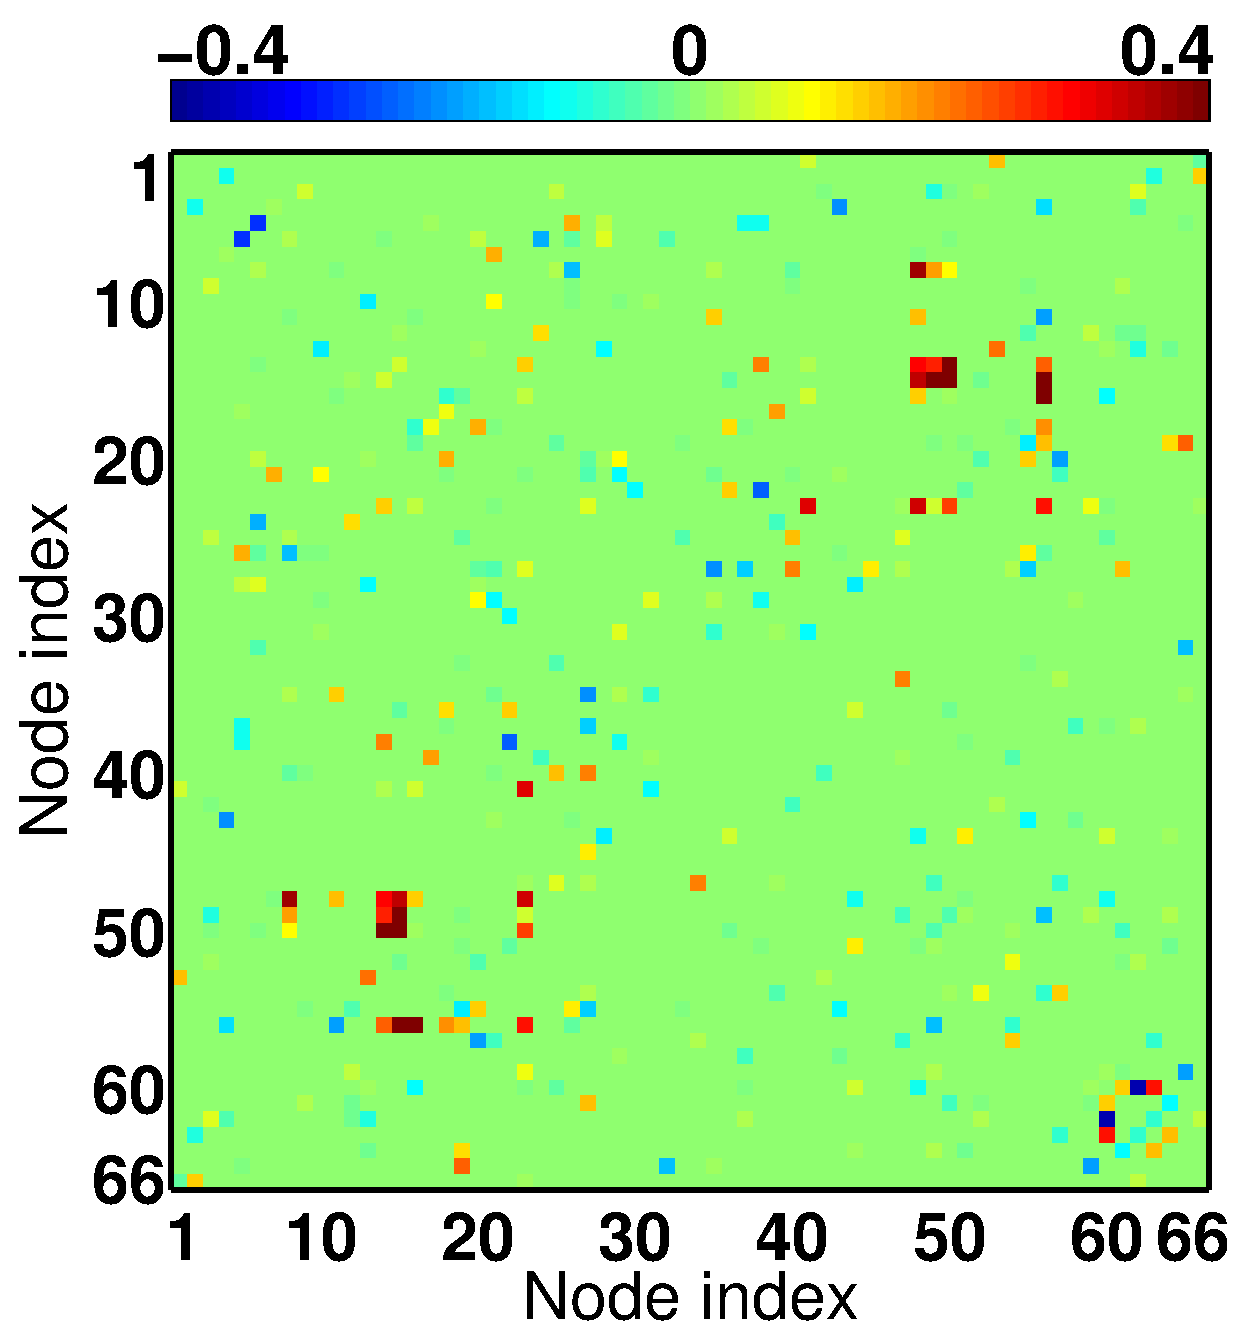
\includegraphics[width=\imwidth]{sim_best_weight_lass100.pdf} &
		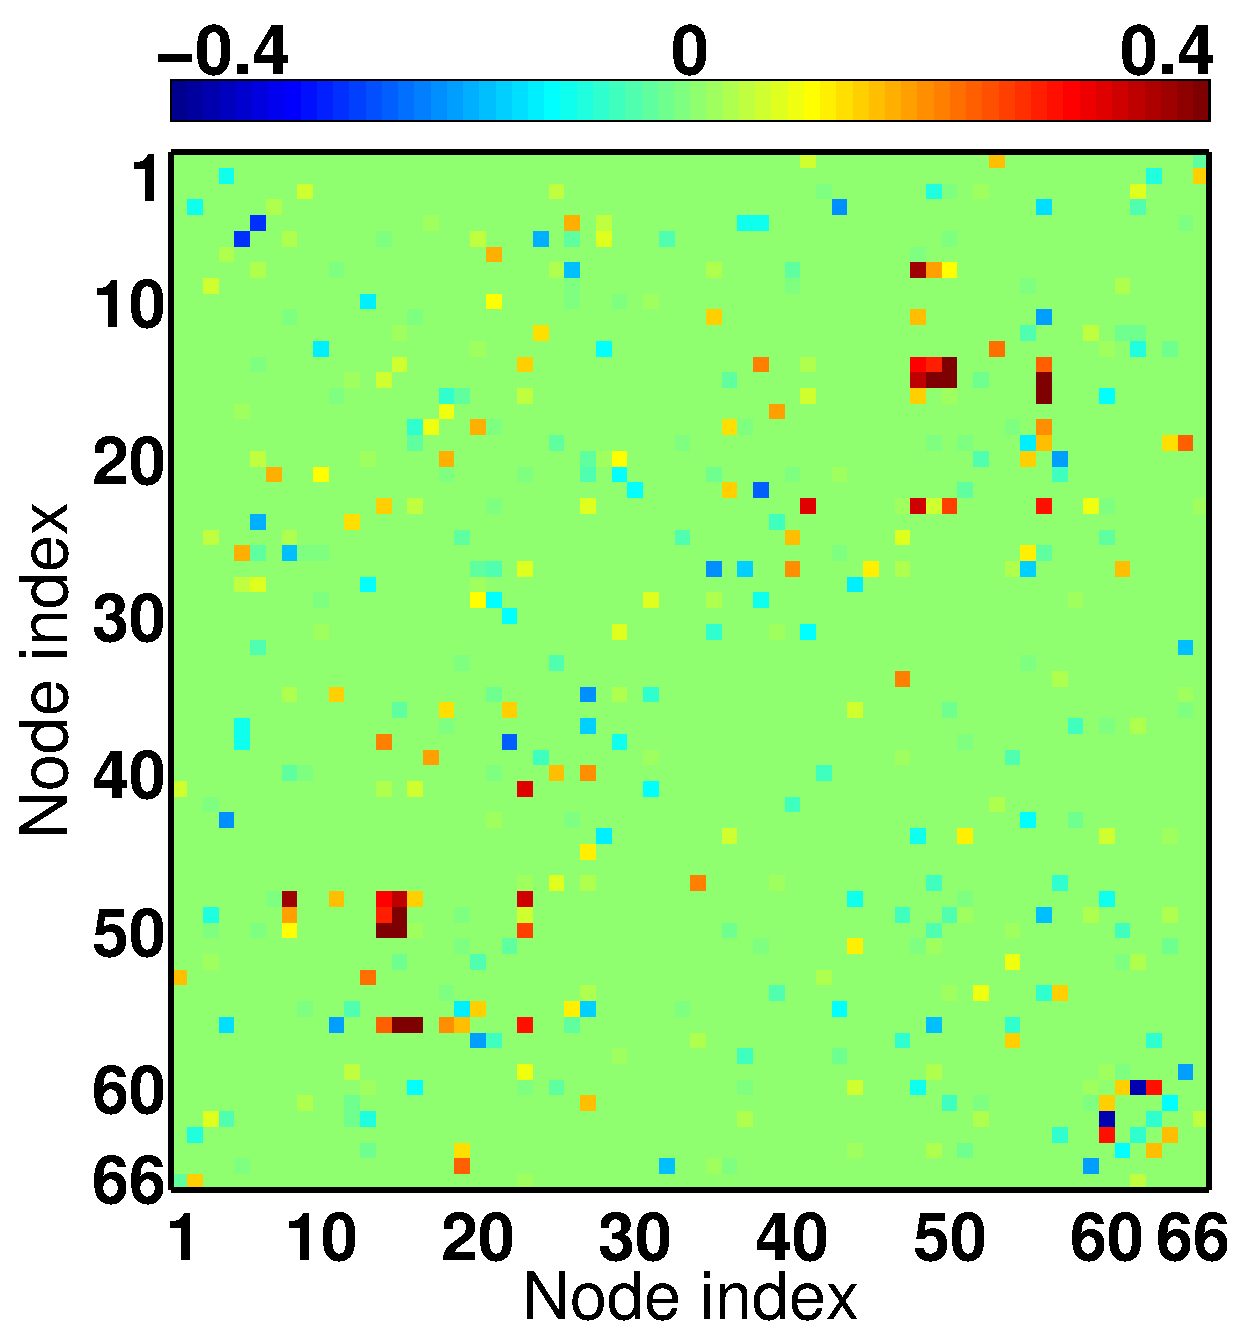
\includegraphics[width=\imwidth]{sim_best_weight_enet100.pdf} &
		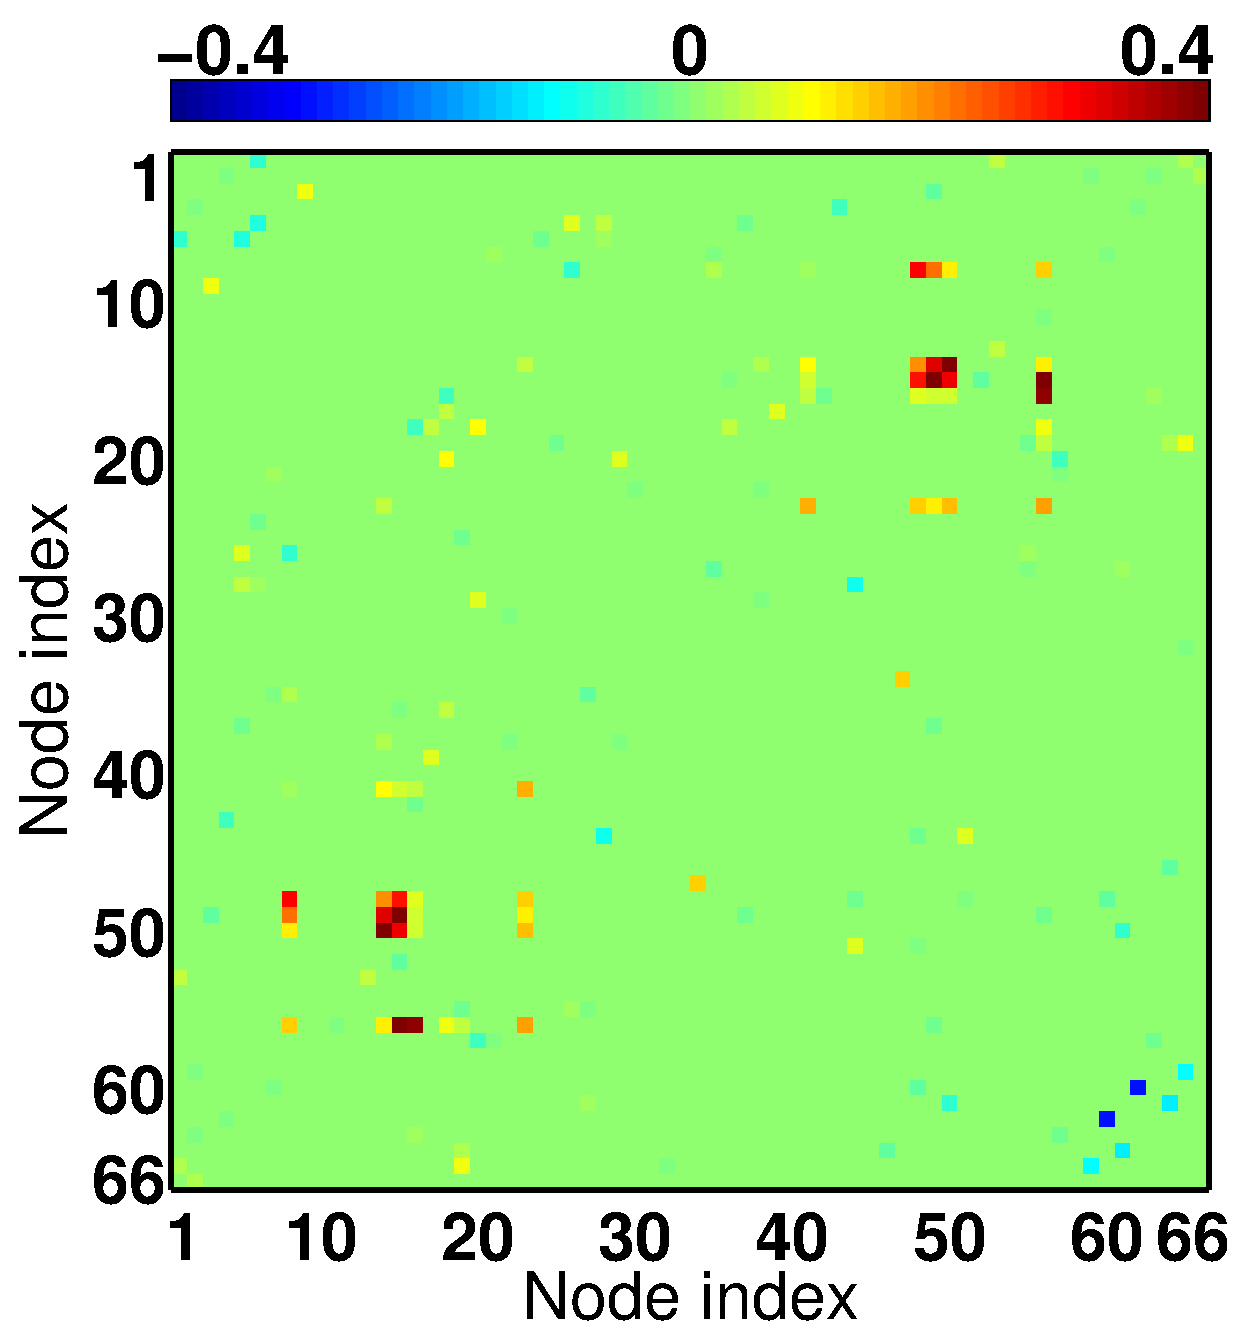
\includegraphics[width=\imwidth]{sim_best_weight_gnet100.pdf} &
		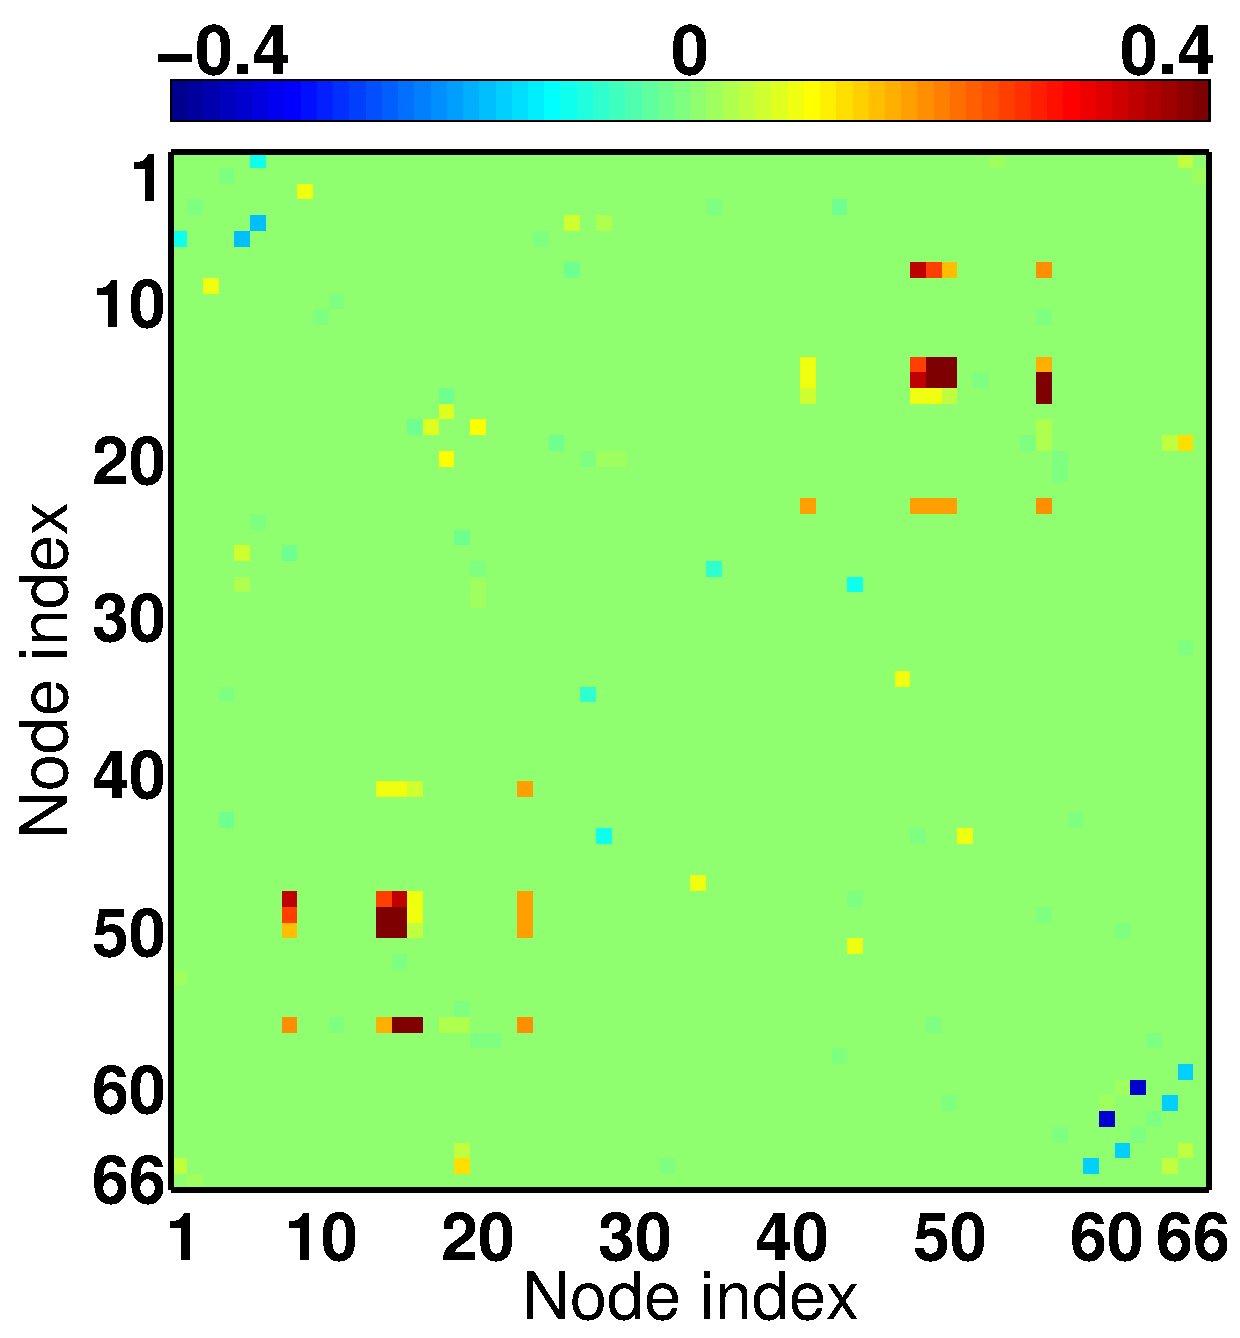
\includegraphics[width=\imwidth]{sim_best_weight_flas100.pdf} \vspace{-3pt}\\
		\small{(a) Lasso} & \small{(b) Elastic-net} & \small{(c) GraphNet} & \small{(d) Fused Lasso} \\
		\footnotesize{(classif. accuracy = $77.0\%$)} &
		\footnotesize{(classif. accuracy = $77.0\%$)} &
		\footnotesize{(classif. accuracy = $85.6\%$)} &
		\footnotesize{(classif. accuracy = $88.2\%$)} \\
	\end{tabular} \vspace{0pt}\\
	\renewcommand{\imwidth} {0.4\linewidth}	
	\begin{subfigure}[b]{\imwidth}\setcounter{subfigure}{4}
		\centering
		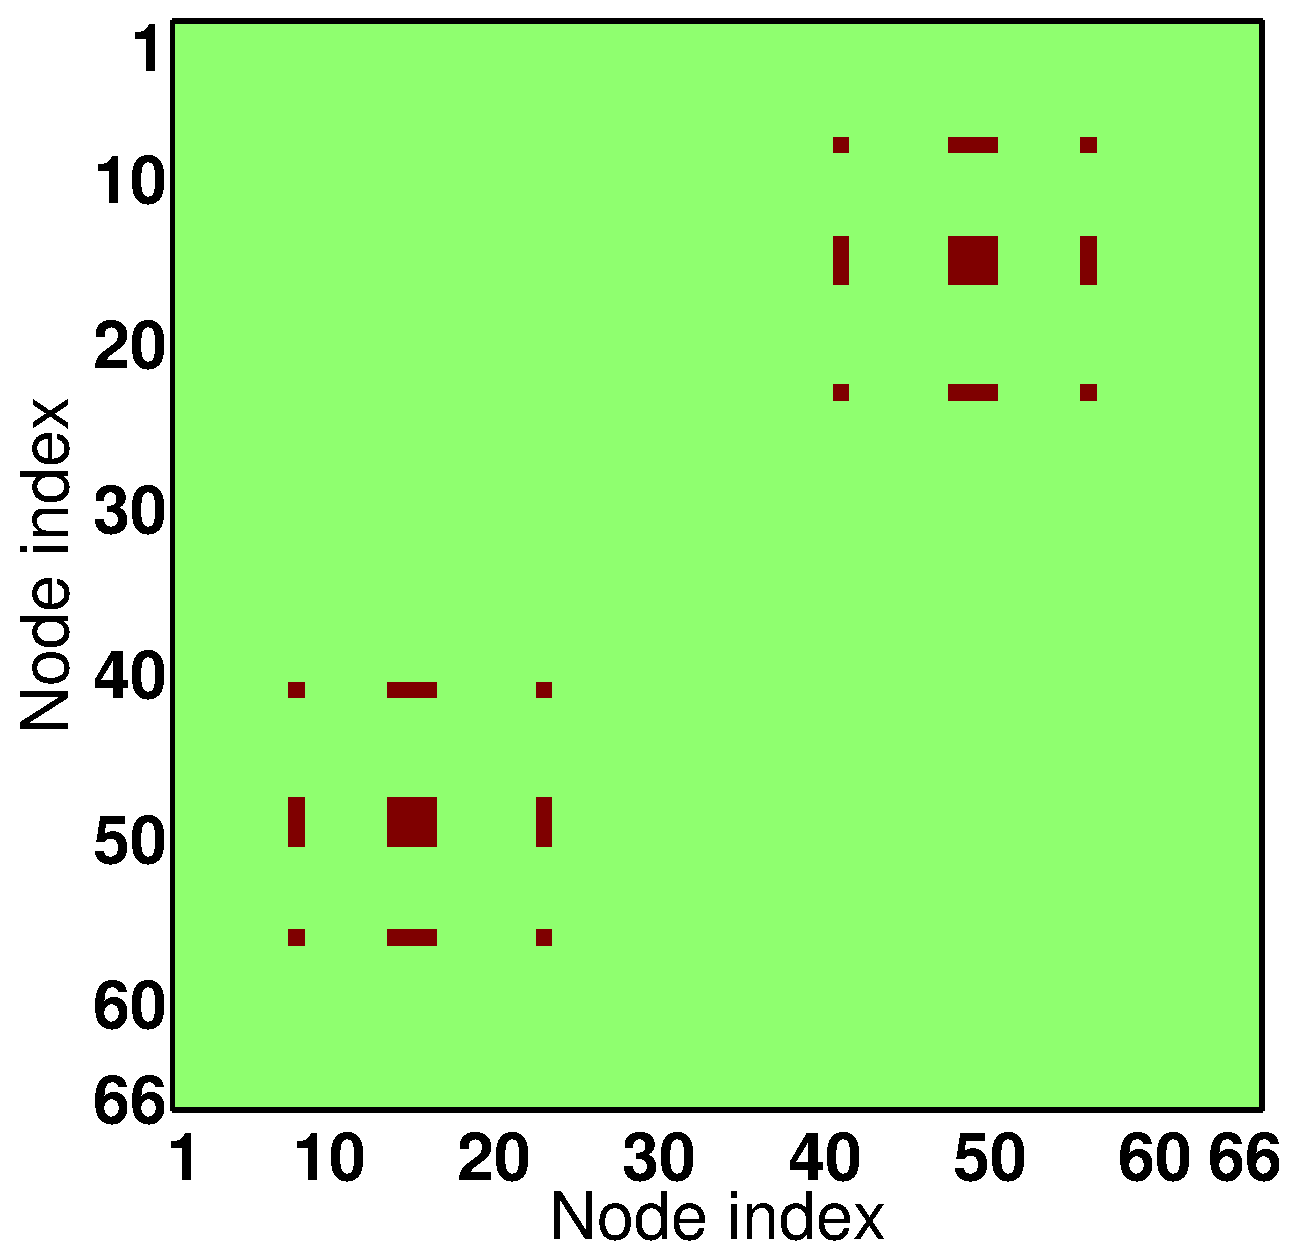
\includegraphics[height=95pt]{sim_best_weight_truth.pdf}
		\vspace{-4pt}\\
		\caption{Support of the \emph{anomalous edges}}
		\label{subfig:sim,edge,truth}
	\end{subfigure}
	\hspace{10pt}
	\begin{subfigure}[b]{\imwidth}
		\centering
		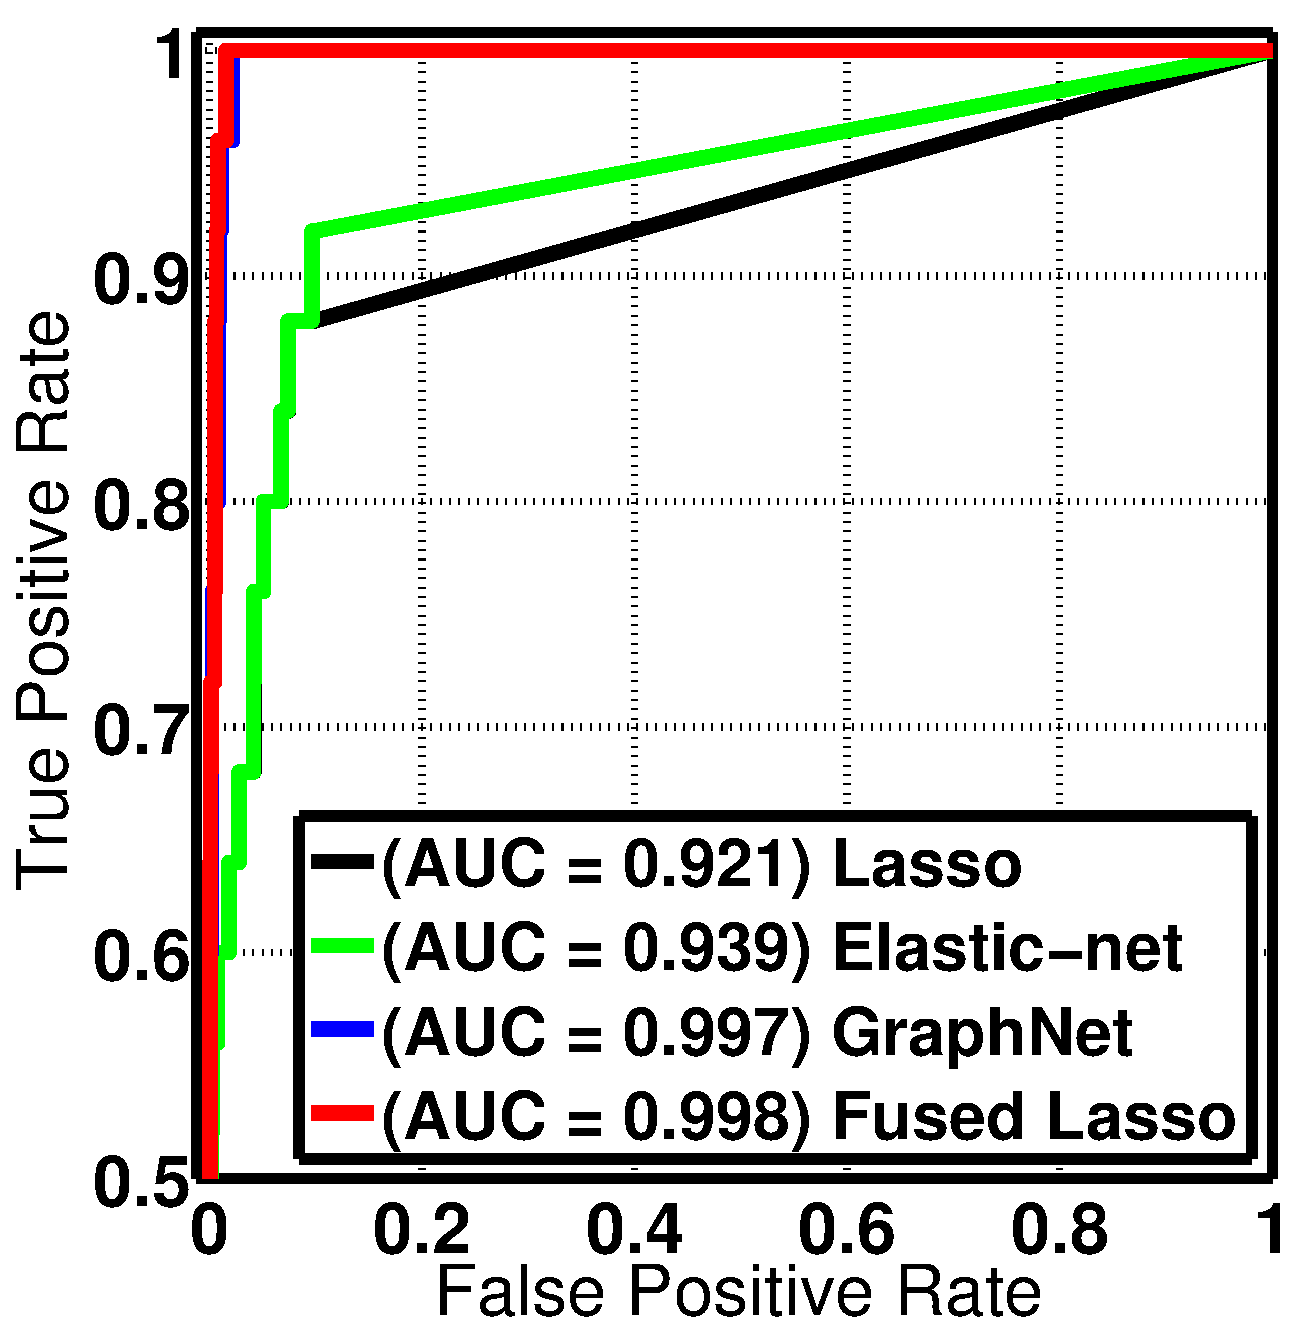
\includegraphics[height=95pt]{sim_best_weight_roc100.pdf}
		\vspace{-4pt}\\
		\caption{ROC (edge identification accuracy)}
		\label{subfig:sim,roc}
	\end{subfigure}
	\vspace{-5pt}\\
	\caption{
		Simulation experiment result: training set consists of $n=100$ samples with $50$ patients and $50$ controls (best viewed in color).  
		\mbox{(a)-(d) Weight} vectors (reshaped into symmetric matrices) estimated from solving the regularized ERM problem~\eqref{eqn:reg,erm} using the hinge-loss and four different regularizers.
		Regularization parameters were tuned via $5$-fold cross-validation on the training set, and classification accuracies were evaluated on a testing set consisting of $500$ samples with $250$ patients and $250$ controls.
		(e) Support matrix indicating the locations of the anomalous edges.
		(f) ROC curve representing the anomalous edge identification accuracy (not classification accuracy) of the four regularizers.
	}
	\label{fig:sim,weight,result}
	\vspace{10pt}
	%=====================================================%
	% simualtion result of the 4 estimation methods:
	% (1) lasso (2) enet (3) gnet (4) flasso
	%=====================================================%
	\renewcommand{\imwidth}  {0.2449\linewidth}
	\renewcommand{\imheight}  {0.2449\linewidth}
	\setlength{\tabcolsep}{1pt} 
	\begin{tabular}{ccccc}
	\multicolumn{4}{c}{{\textbf{\normalsize{Classification accuracy}}}} \vspace{0pt} \\
	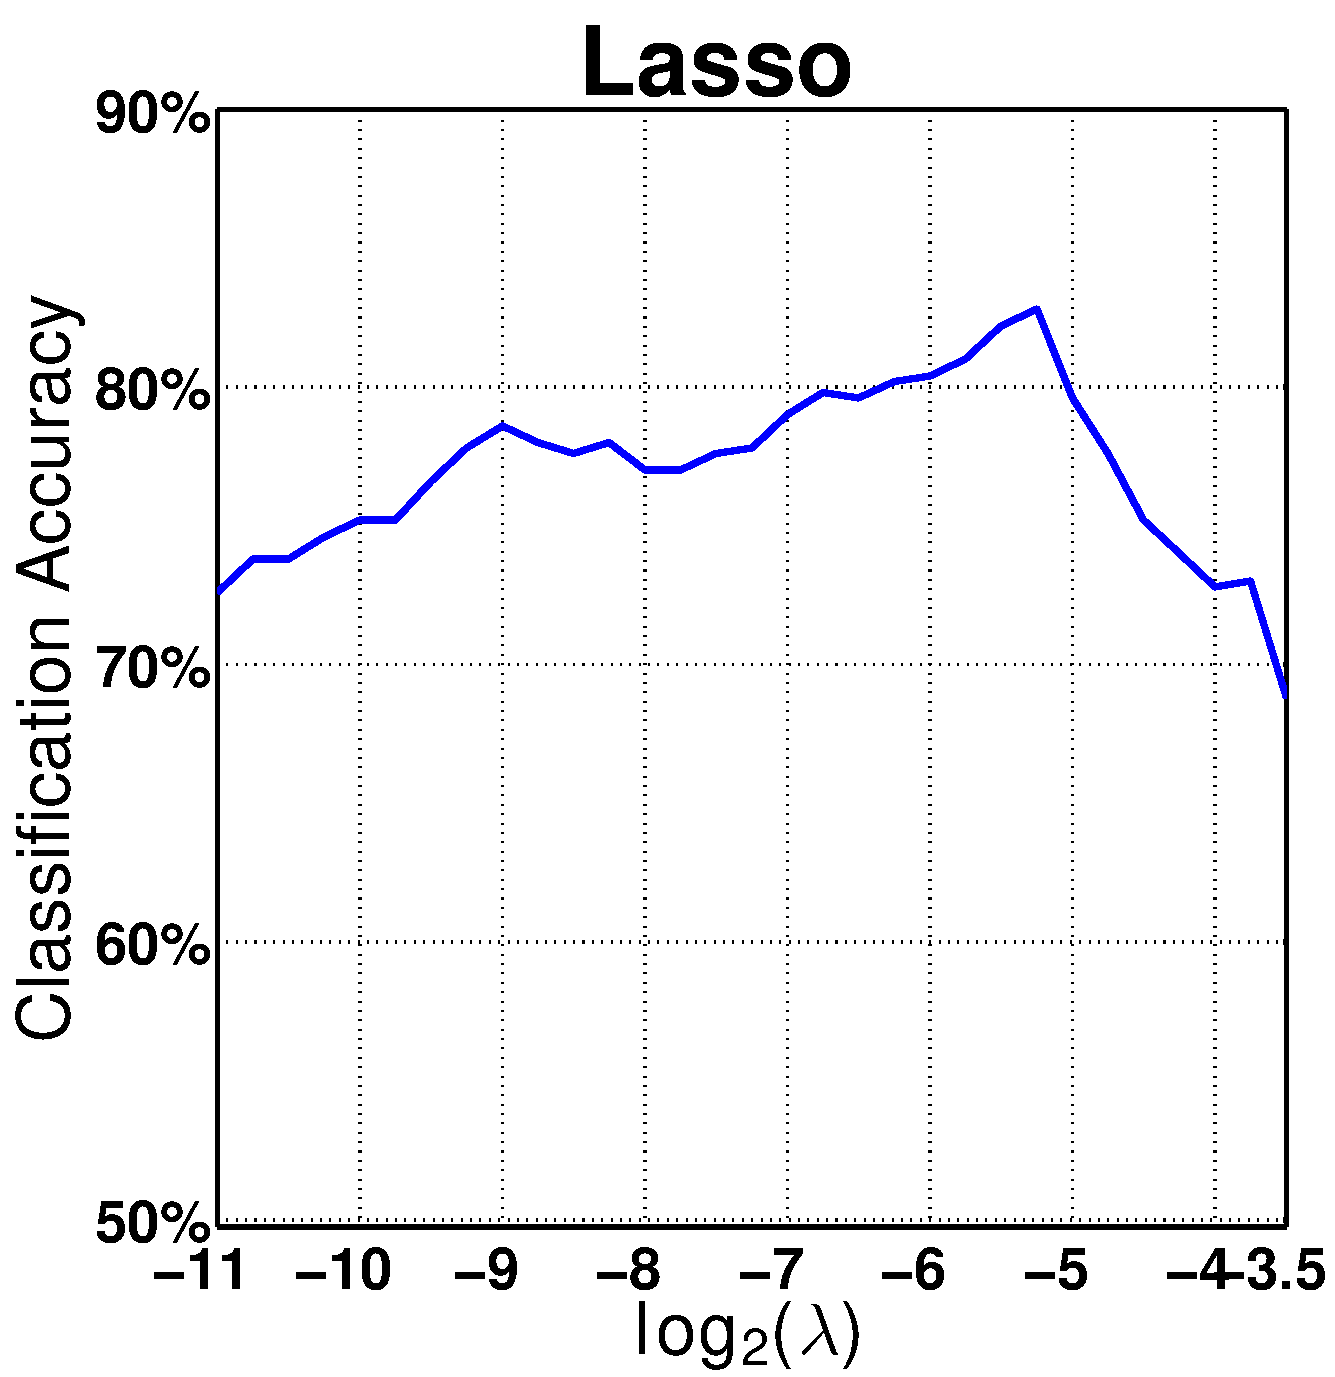
\includegraphics[height=\imheight,width=\imwidth]{sim_gridsearch_lass_acc100.pdf} &
	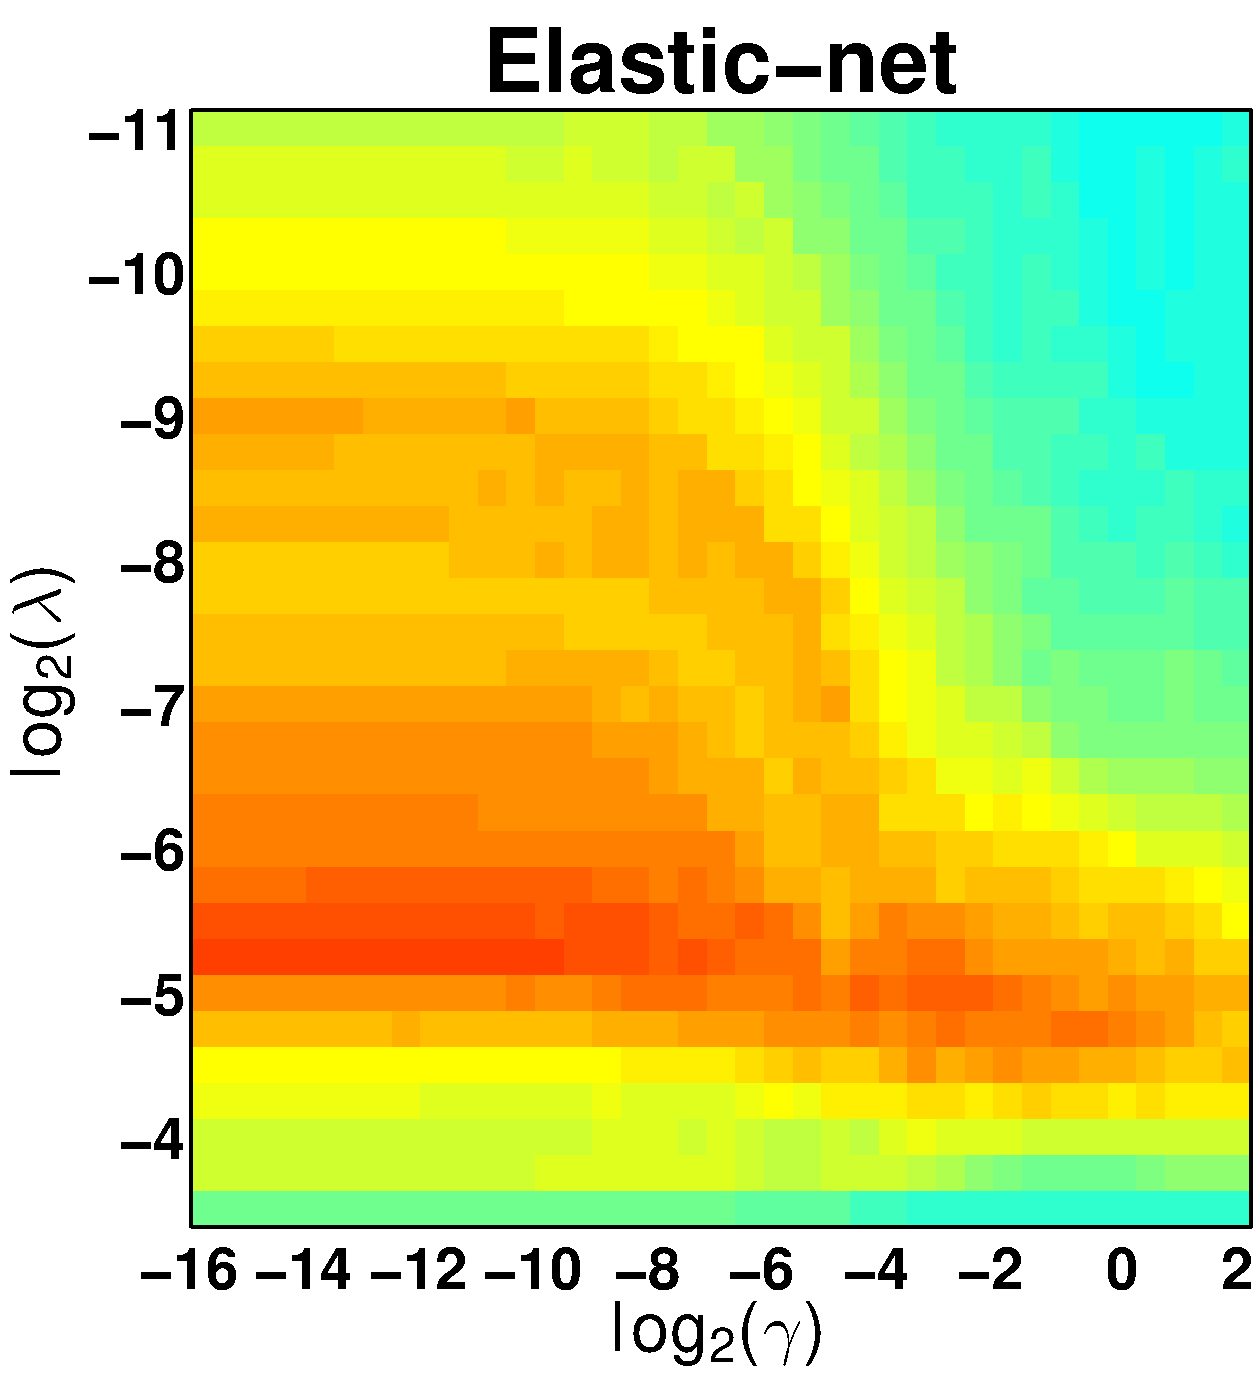
\includegraphics[height=\imheight,width=\imwidth]{sim_gridsearch_enet_acc100.pdf} &
	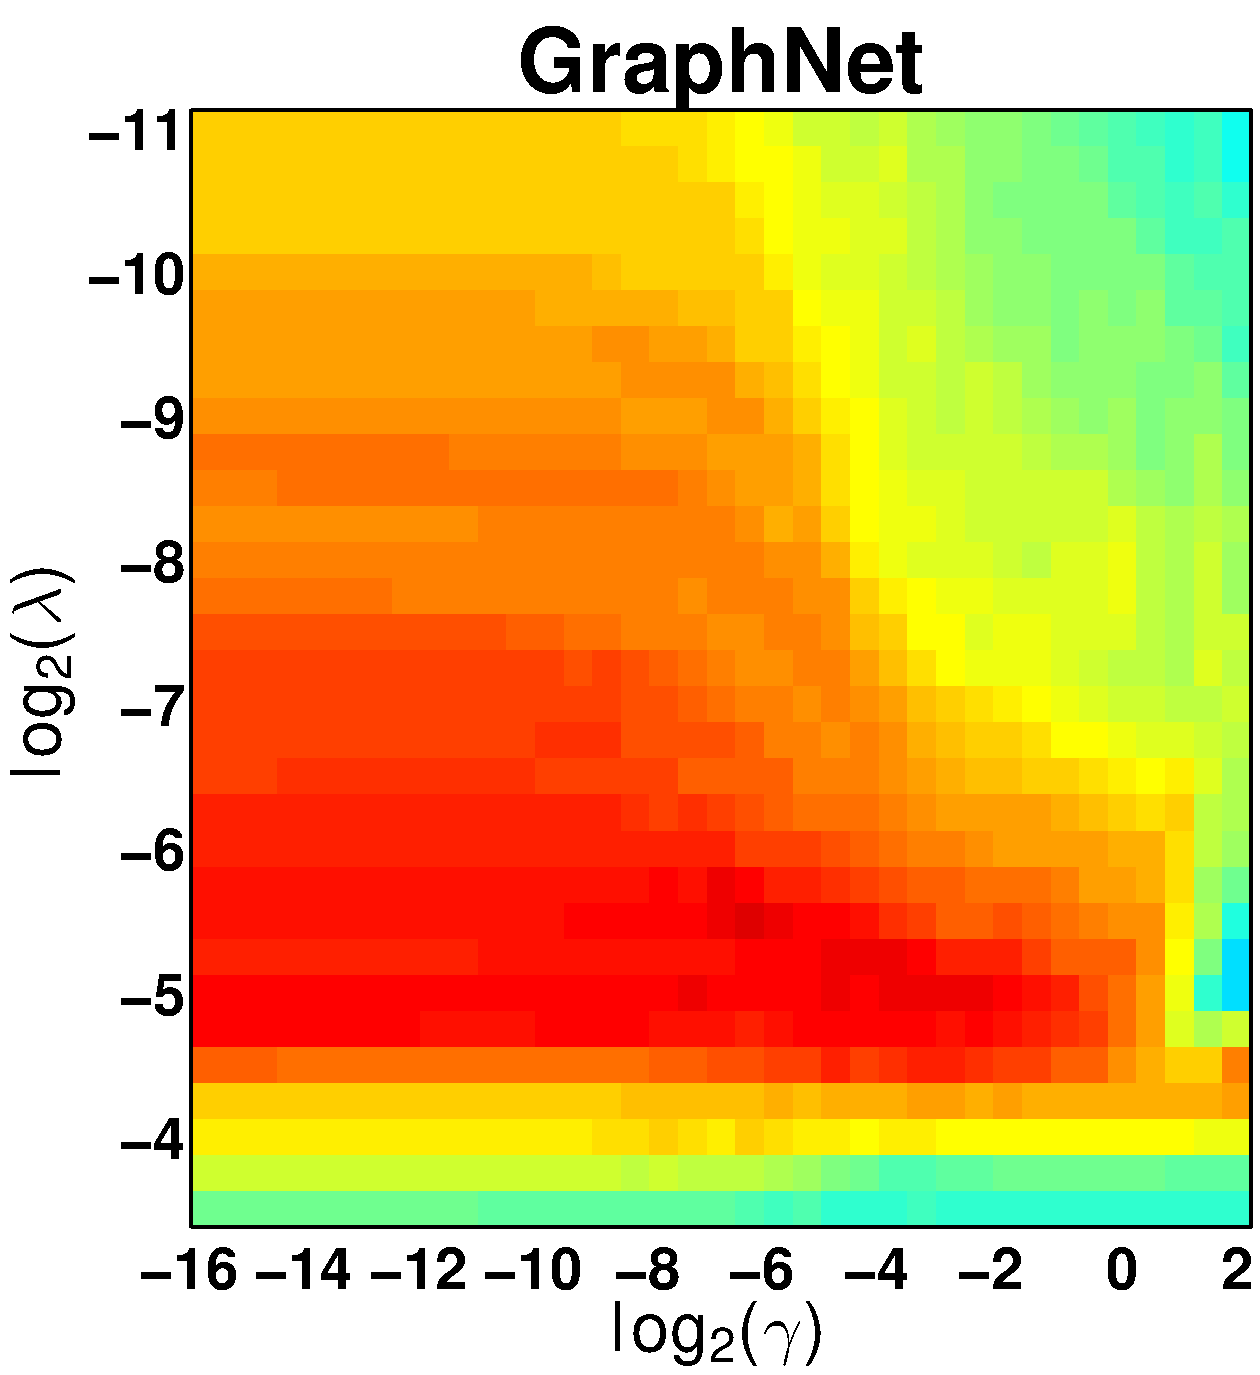
\includegraphics[height=\imheight,width=\imwidth]{sim_gridsearch_gnet_acc100.pdf} &
	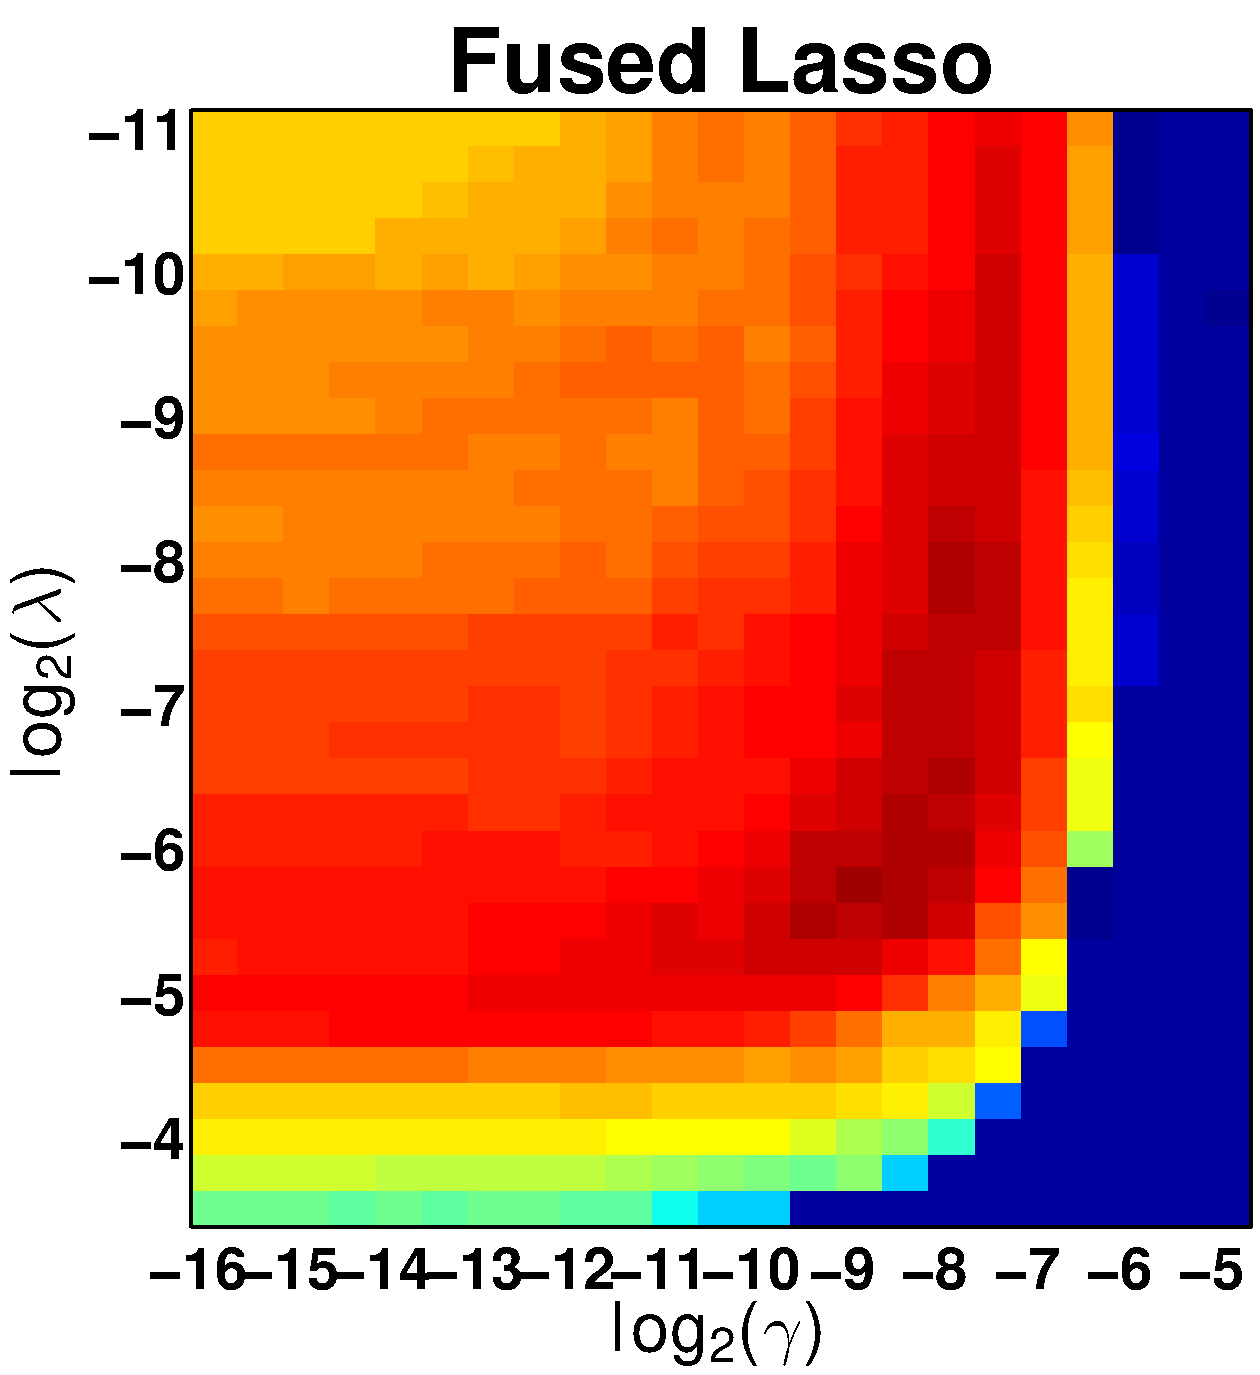
\includegraphics[height=\imheight,width=\imwidth]{sim_gridsearch_flas_acc100.pdf} &
	\raisebox{0.02585\linewidth}{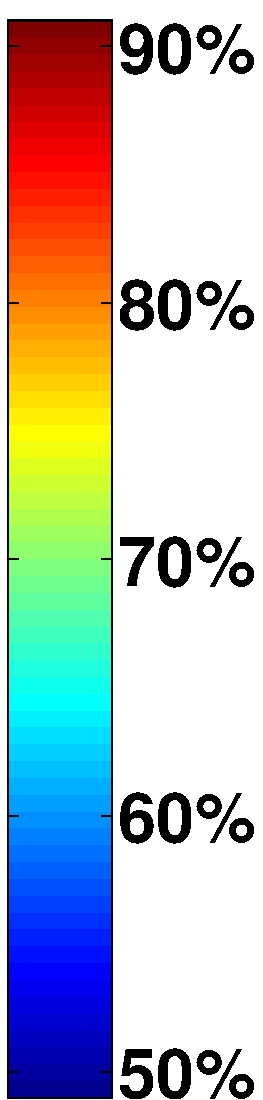
\includegraphics[height=0.2035\linewidth]{sim_gridsearch_crangeACC100.pdf}} 
	\vspace{1pt}\\
	%%
	\multicolumn{4}{c}{{\textbf{\normalsize{Sparsity level (number of features)}}}} \vspace{0pt}\\
	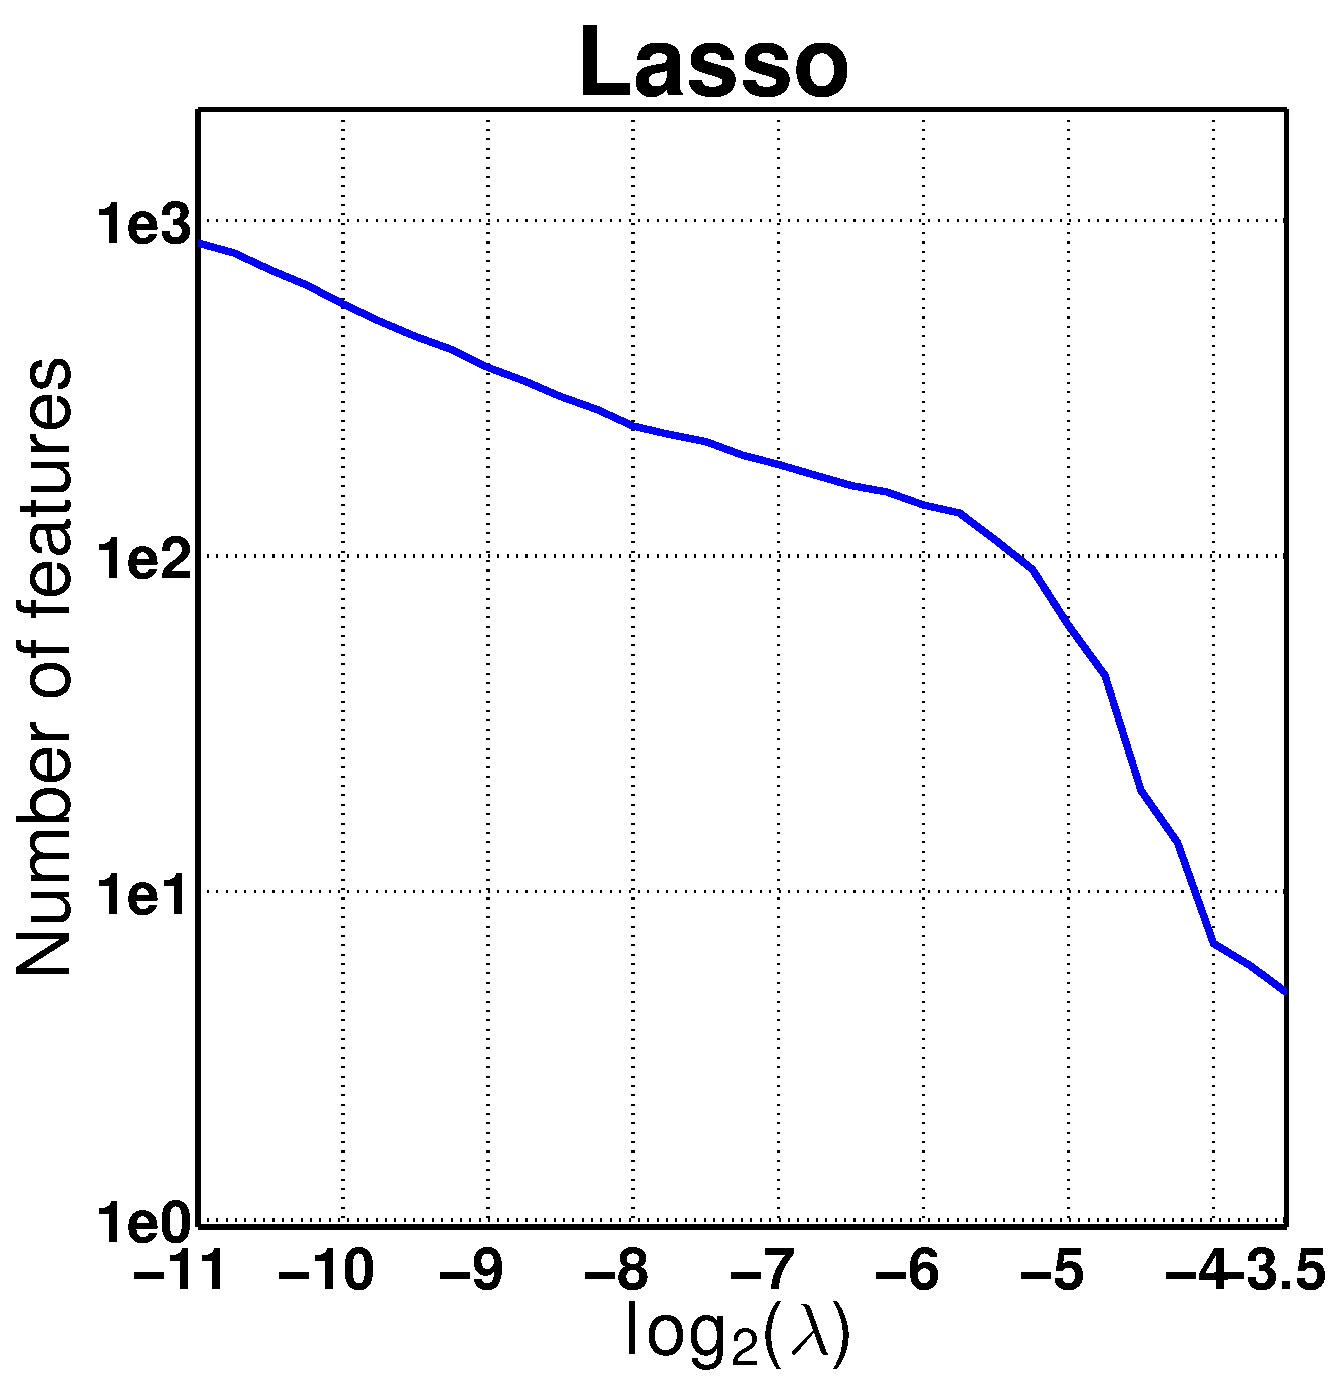
\includegraphics[height=\imheight,width=\imwidth]{sim_gridsearch_lass_nnz100.pdf} &
	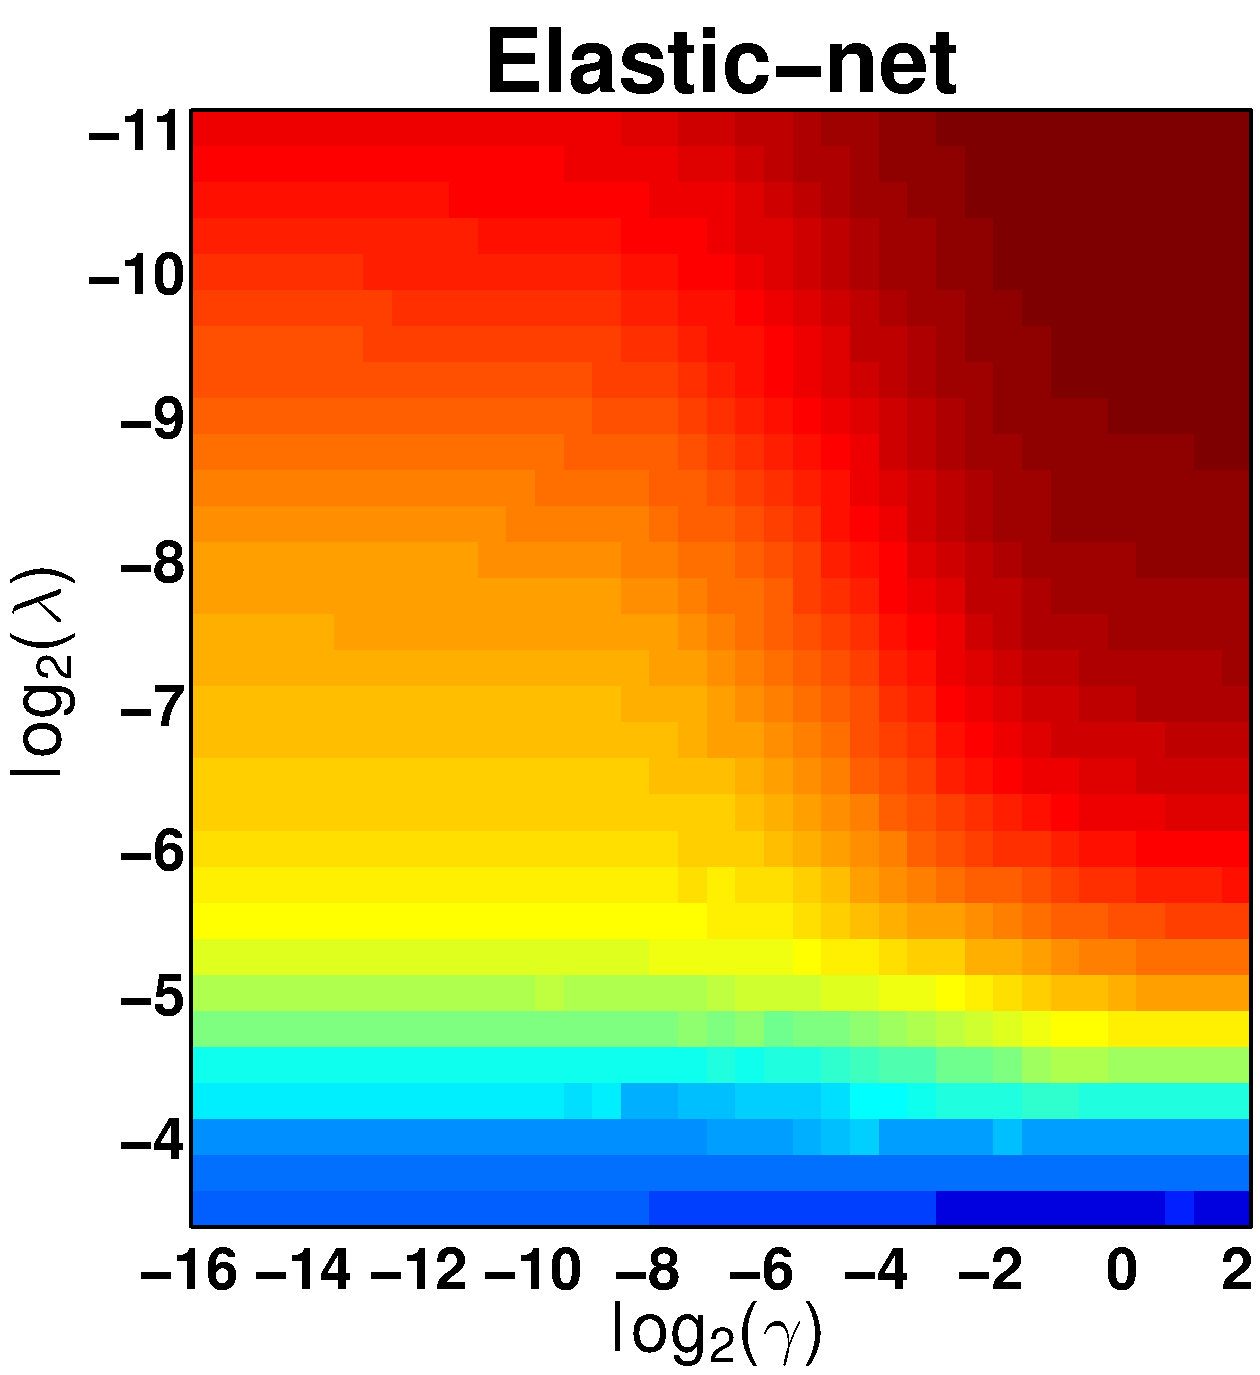
\includegraphics[height=\imheight,width=\imwidth]{sim_gridsearch_enet_nnz100.pdf} &
	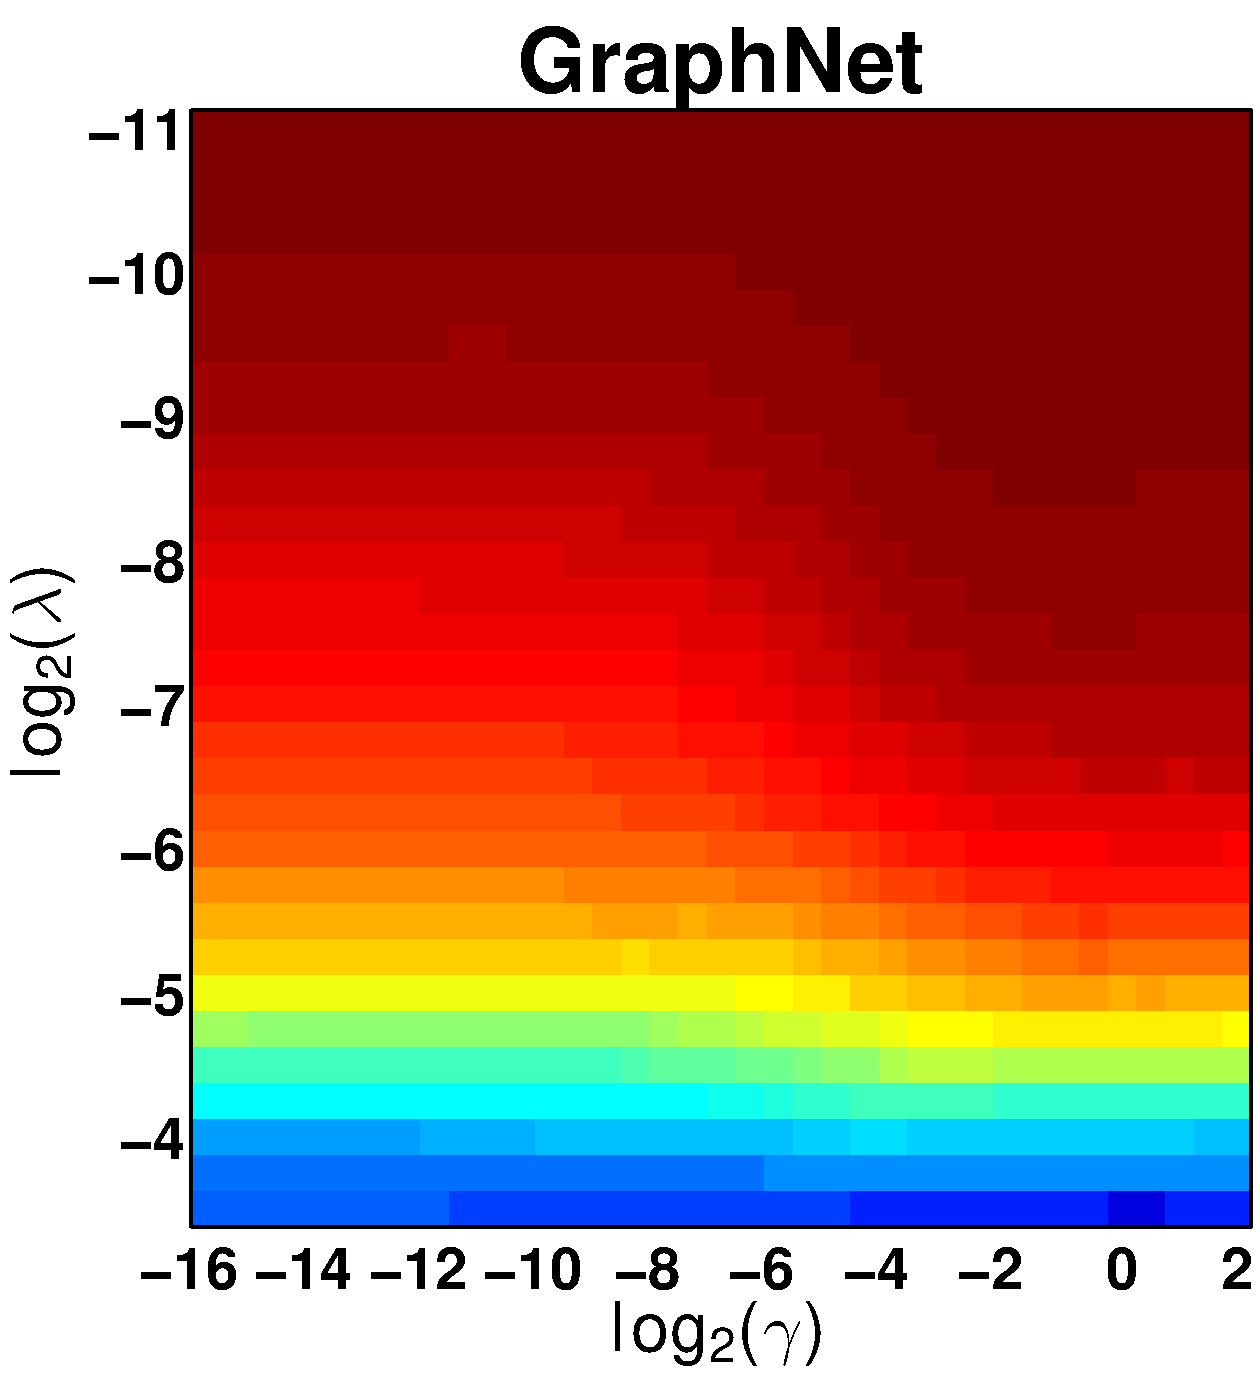
\includegraphics[height=\imheight,width=\imwidth]{sim_gridsearch_gnet_nnz100.pdf} &
	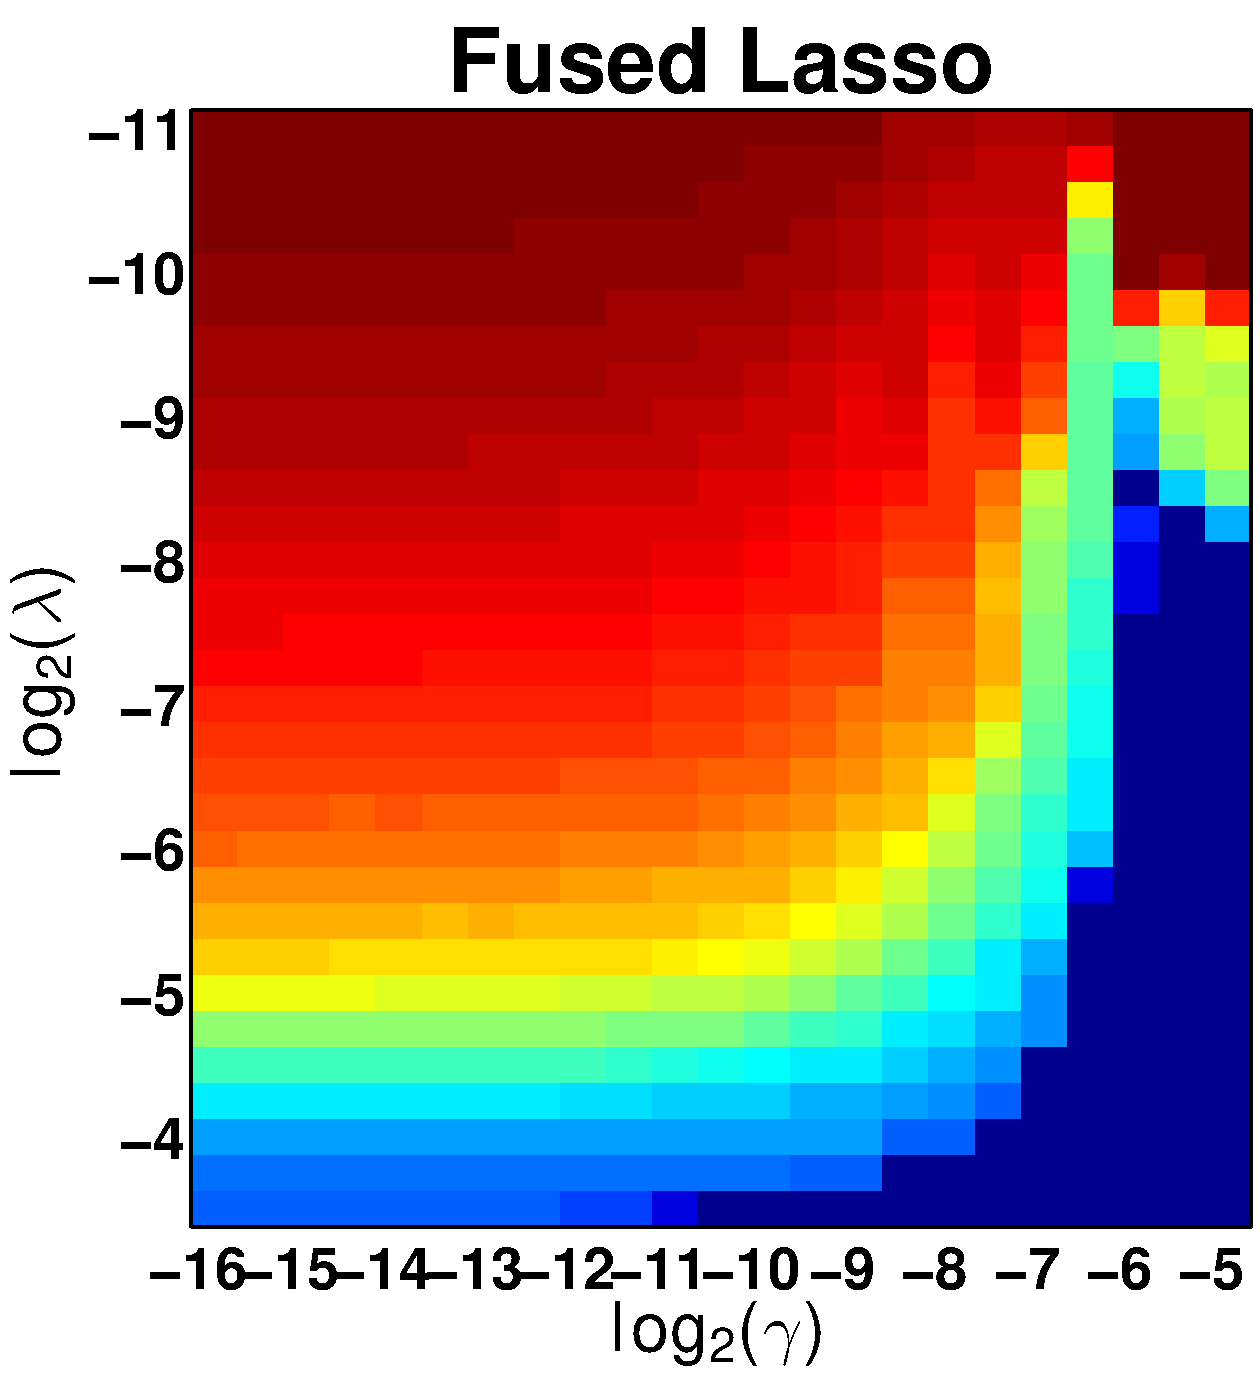
\includegraphics[height=\imheight,width=\imwidth]{sim_gridsearch_flas_nnz100.pdf} &
	\hspace{0pt}\raisebox{0.021423\linewidth}{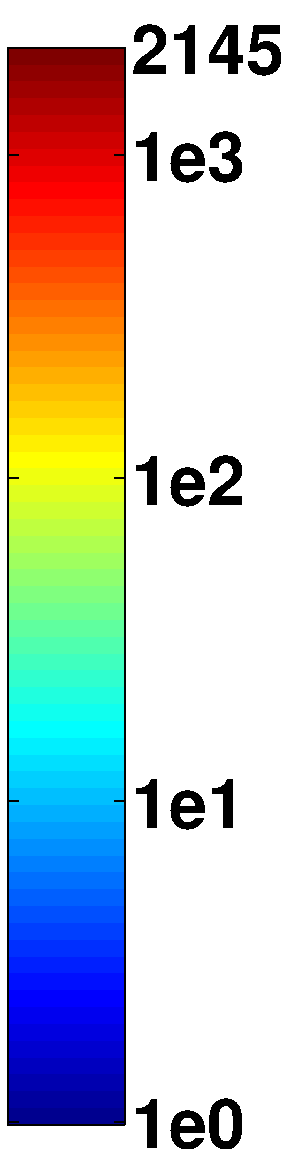
\includegraphics[height=0.213\linewidth]{sim_gridsearch_crangeNNZ100.pdf}} \\
	\end{tabular}
	\vspace{-10pt}\\
	\caption{Grid search result for the simulation experiment (best viewed in color).
	 	All classifiers were learned using $100$ training samples consisting of $50$ patients and $50$ controls.	 	
		\textbf{Top row}: classification accuracy as a function of the regularization parameters $\{\lambda,\gamma\}$ (evaluated from $500$ testing samples consisting of $250$ patients and $250$ controls).
		\textbf{Bottom row}: the number of features selected as a function of the regularization parameters $\{\lambda,\gamma\}$.
	}
	\label{fig:sim,grid,ntr}
\end{figure}
%%%%%%%%%%%%%%%%%%%%%%%%%%%%%%%%%%%%%%%%%%%%%%%%%%%%%%%%%
%%%%%%%%%%%%%%%%%%%%%%%%%%%%%%%%%%%%%%%%%%%%%%%%%%%%%%%%%%%%%%%%%%%%%%%%%%%
The top row of Fig.~\ref{fig:sim,weight,result} displays the estimated weight vectors, and the corresponding testing classification accuracies are reported under the subcaptions. 
Here, the fused Lasso regularized SVM yielded the best classification accuracy at $88.2\%$ using $92$ features, followed by $85.6\%$ from GraphNet which used $104$ features; Lasso and Elastic-net both achieved $77.0\%$ classification accuracy using $230$ and $232$ features respectively.
However, a perhaps more interesting observation is that fused Lasso and GraphNet were able to recover the structure of the \emph{anomalous edges} much more clearly than Lasso and Elastic-net; this can be seen by comparing the weight vectors estimated by the four regularizers with the support of the anomalous edges displayed in Fig.~\ref{subfig:sim,edge,truth}.
While Lasso and Elastic-net yielded weight vector estimates with salt-and-pepper patterns that are difficult to interpret, the weight vector estimates for fused Lasso and GraphNet closely resembles the  structure of the \emph{anomalous edges}.
To quantify the regularizers' ability to identify the discriminative edges, we generated a receiver operating characteristic (ROC) curve by thresholding the absolute value of the elements of the estimated weight vector.
The resulting ROC curve for the four regularizers are plotted in Fig.~\ref{subfig:sim,roc}; we emphasize that this ROC curve summarizes the regularizers' ability to identify the informative edges, and does not represent classification accuracy.
From this ROC curve, we see that fused Lasso and GraphNet attain the best performances, achieving a nearly perfect \emph{area under the curve} (AUC) value of $0.998$ and $0.997$ respectively, whereas the AUC value for Lasso and Elastic-net were $0.921$ and $0.939$ respectively.
In short, Fig.~\ref{fig:sim,weight,result}a-f demonstrate that fused Lasso and GraphNet not only improved classification accuracy, but also exhibited superior performance in recovering the discriminatory edges with respect to their non-spatially informed counterparts, Lasso and Elastic-net.

In our next analysis, we studied how classification accuracy and sparsity (\ie, number of features selected) behave as a function of the regularization parameters $\{\lambda,\gamma\}$.
For this, we conducted a grid search over the same range of $\lambda$ and $\gamma$ values presented above, but the classifiers were trained over the entire training set.
Classification accuracy was evaluated on the same testing set as the above experiment.
The result of the grid search is presented in Fig.~\ref{fig:sim,grid,ntr}, where the top row plots the testing classification accuracy and the bottom row plots the number of features selected, both as a function of the regularization parameters $\{\lambda,\gamma\}$.

%%%%%%%% TABLE & PLOT OF CLASSICATION ACC IN SIMU %%%%%%%
%*************************************************************************%
% simulation classification accuracy: comparison result
% - script looks unholy, but this ensures a table and figure to be displayed together on top of the page
% - http://tex.stackexchange.com/questions/47900/place-a-minipage-on-the-top-of-a-page
% - http://tex.stackexchange.com/questions/55337/how-to-use-figure-inside-a-minipage
%%%%%%%%%%%%%%%%%%%%%%%%%%%%%%%%%%%%%%%%%%%%%%%%%%%%%%%%%%%%%%%%%%%%%%%%%%%
\begin{figure}[!t]
\noindent
\begin{minipage}{\textwidth}
%======= figure of classification result in simulation =====%
	\centering
	\renewcommand{\imwidth}  {0.35\linewidth}
	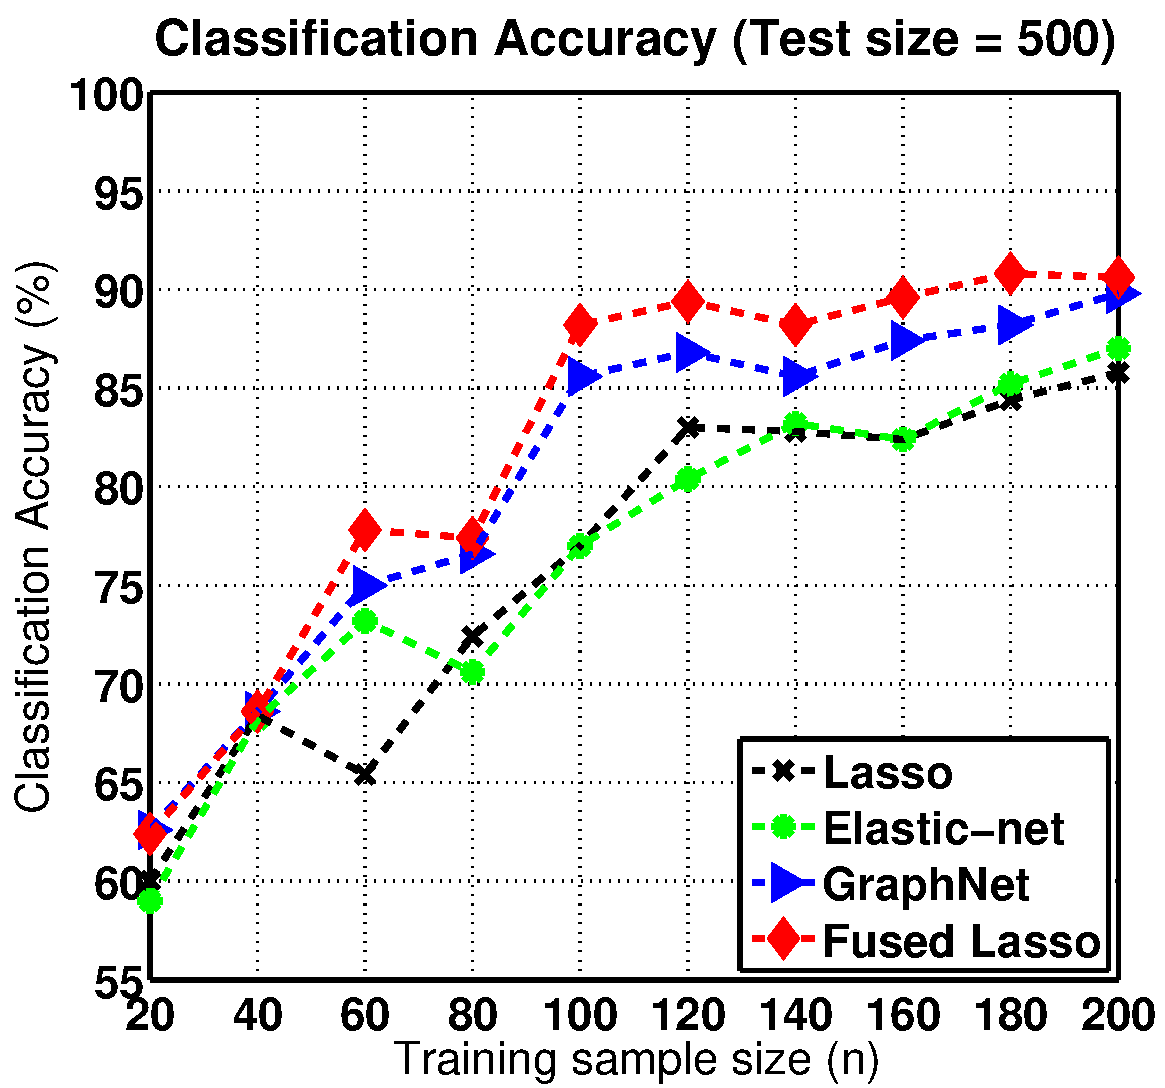
\includegraphics[width=\imwidth]{sim_samp_complexity.pdf} 
	\captionof{figure}{
		The testing classification accuracy of the different regularizers as a function as a number of training samples~$n$ in the simulation experiment.  
		Regularization parameters were tuned via $5$-fold cross-validation on the training set.  
		The testing set consists of $500$ samples with $250$ patients and $250$ controls.
		Table~\ref{table:sim,acc} reports the actual numbers.
	}
	 \label{fig:sim,acc,plot}
\vspace{10pt}
%======= table of classification result in simulation =====%
	\setlength{\tabcolsep}{4.5pt}  %<- controls spacing between tab elements
	\begin{tabular}{c||c|c|c|c|c|c|c|c|c|c}
		\multicolumn{1}{l}{} &	\multicolumn{10}{c}{Testing Classification accuracy ($n$ = training sample size, $500$ = test size)}\\
		\hline
		\textbf{\small{Regularizer}} &
			\small{$n$=20} & \small{$n$=40} &\small{$n$=60}& \small{$n$=80} & \small{$n$=100} & \small{$n$=120} & \small{$n$=140} & \small{$n$=160} &\small{$n$=180} & \small{$n$=200} \\
		\hline\hline
		\textbf{\small{Lasso}} &
			\small{60.0\%}& \small{68.4\%}& \small{65.4\%}& \small{72.4\%}& \small{77.0\%}& \small{83.0\%}& \small{82.8\%}& \small{82.4\%}& \small{84.4\%}& \small{85.8\%}\\
		\textbf{\small{Elastic-net}} & 
			\small{59.7\%}& \small{68.2\%}& \small{73.2\%}& \small{70.6\%}& \small{77.0\%}& \small{80.4\%}& \small{83.2\%}& \small{82.4\%}& \small{85.2\%}& \small{87.0\%}\\
		\textbf{\small{GraphNet}} &
			\textbf{\small{62.6\%}}& \textbf{\small{68.6\%}}& \small{75.0\%}& \small{76.6\%}& \small{85.6\%}& \small{86.8\%}& \small{85.6\%}& \small{87.4\%}& \small{88.2\%}& \small{89.8\%}\\
		\textbf{\small{Fused Lasso}} &
			\small{62.4\%}& \textbf{\small{68.6\%}}& \textbf{\small{77.8\%}}& \textbf{\small{77.4\%}}& \textbf{\small{88.2\%}}& \textbf{\small{89.4\%}}& \textbf{\small{88.2\%}}& \textbf{\small{89.6\%}}& \textbf{\small{90.8\%}}& \textbf{\small{90.6\%}}\\
		\hline
	\end{tabular}
	\captionof{table}{
		The testing classification accuracy of the different regularizers as a function as a number of training samples~$n$ in the simulation experiment (the best classification accuracy for each $n$ is denoted in bold font).
		See Fig.~\ref{fig:sim,acc,plot} for a plot of this result.
	}
	\label{table:sim,acc}
\end{minipage}
\end{figure}
%%%%%%%%%%%%%%%%%%%%%%%%%%%%%%%%%%%%%%%%%%%%%%%%%%%%%%%%%

To further study the performance of our method, we next conducted a \emph{sample complexity analysis} \citep{Gramfort:2011}, where we studied how the classification accuracy of the four regularizers behaved as a function of the training sample size $n$.
This was done by repeating our earlier experiment of tuning the regularization parameters via $5$-fold cross-validation on the training set, but here we varied the training sample size over the range $n\in\{20,40,60,\dots,200\}$; the same testing set of size $500$ was used throughout for evaluating the classification accuracy.
Note the labels are balanced for all datasets, \ie, the training set consists of $n/2$ patients and $n/2$ controls, and similarly the testing set consists of $250$ patients and $250$ controls.
The result of this experiment is reported in Fig.~\ref{fig:sim,acc,plot} and Table~\ref{table:sim,acc}.
A key observation from this analysis is that the classification accuracy for GraphNet and fused Lasso consistently outperformed Lasso and Elastic-net, which can be attributed to the spatial information injected by these spatially-informed regularizers.
Overall, fused Lasso yielded the best classification accuracy.

It is important to note that the inclusion of the anomalous node clusters in the data generating process certainly favors fused Lasso and GraphNet.
However, we remind the readers that these anomalous node clusters are not some arbitrary structures we introduced to favor the spatially-informed regularizers, but are motivated from the ``patchiness assumption'' of brain disorders, a neuroscientific viewpoint which we discuss in detail in Sec.~\ref{subsec:why,flasso}.
The results from the simulation experiments confirm the intuition that if the ``patchiness assumption'' of brain disorders holds true, spatially-informed classifiers can be a powerful tool for recovering relevant biosignatures.

%===================================================================%
% 			Real data experiment results
%===================================================================%
\subsection{Results on resting state fMRI data from a schizophrenia dataset}
\label{subsec:result,real,data}
In this experiment, we examined the performance of linear classifiers trained using regularized ERM \eqref{eqn:reg,erm} with the hinge-loss, and three regularizers were subject to comparison: Elastic-net, GraphNet, and fused Lasso.  
The study involved $121$ participants, consisting of $54$ schizophrenic subjects (SZ) and $67$ healthy controls (HC).
We adopt the convention of letting $y=+1$ indicate SZ and $y=-1$ indicate HC subjects.
The ADMM algorithm was terminated when the tolerance level~\eqref{eqn:admm,termin} fell below $\varepsilon=4\times 10^{-3}$ or the algorithm reached $400$ iterations.
Empirically, we found the algorithm to converge at around $180\mytilde 300$ iterations.
For the two regularization parameters, we conducted a two-dimensional grid search: the \ellone regularization parameter $\lambda\geq 0$ was searched over the range $\lambda\in\{2^{-20},2^{-19},\cdots,2^{-3}\}$ for all three regularizers, and the second regularization parameter $\gamma\geq 0$ was searched over $\gamma\in\{2^{-20},2^{-19},\cdots,2^{3}\}$ for Elastic-net and GraphNet and $\gamma\in\{2^{-20},2^{-19},\cdots,2^{-3}\}$ for fused Lasso.
Ten-fold cross-validation to evaluate the generalizability of the classifiers.
Furthermore, we analyzed the sparsity level achieved during the grid search by computing the average number of features selected across the cross-validation folds.

The resulting testing classification accuracy and sparsity level for different combinations of $\{\lambda,\gamma\}$ are rendered as heatmaps in Fig.~\ref{fig:grid,search}.
The general trend observed from the grid search is that for all three regularization methods, the classification accuracy improved as more features entered the model.
We observed the same trend when using other loss functions as well, specifically the truncated-least squares loss and the huberized-hinge loss (using $\delta=0.5$) function.
Although this behavior may be somewhat surprising, it has been reported that in the $p\gg n$ setting, the unregularized SVM often performs just as well as the best regularized case, and accuracy can degrade when feature pruning takes place (see Ch.18 in \cite{Hastie:2009:book}).

%=========== Grid search result for the 3 methods =============
\newcommand{\addhspace}{\hspace{0.04\linewidth}}
\begin{figure}[t]
	\setlength{\tabcolsep}{1pt} 
	\renewcommand{\imwidth}  {0.3\linewidth}
	\renewcommand{\imheight}  {0.3105\linewidth}	
	\begin{tabular}{cccc}	
	\multicolumn{4}{c}{{\textbf{\large{Classification accuracy}}}} \vspace{0pt} \\
	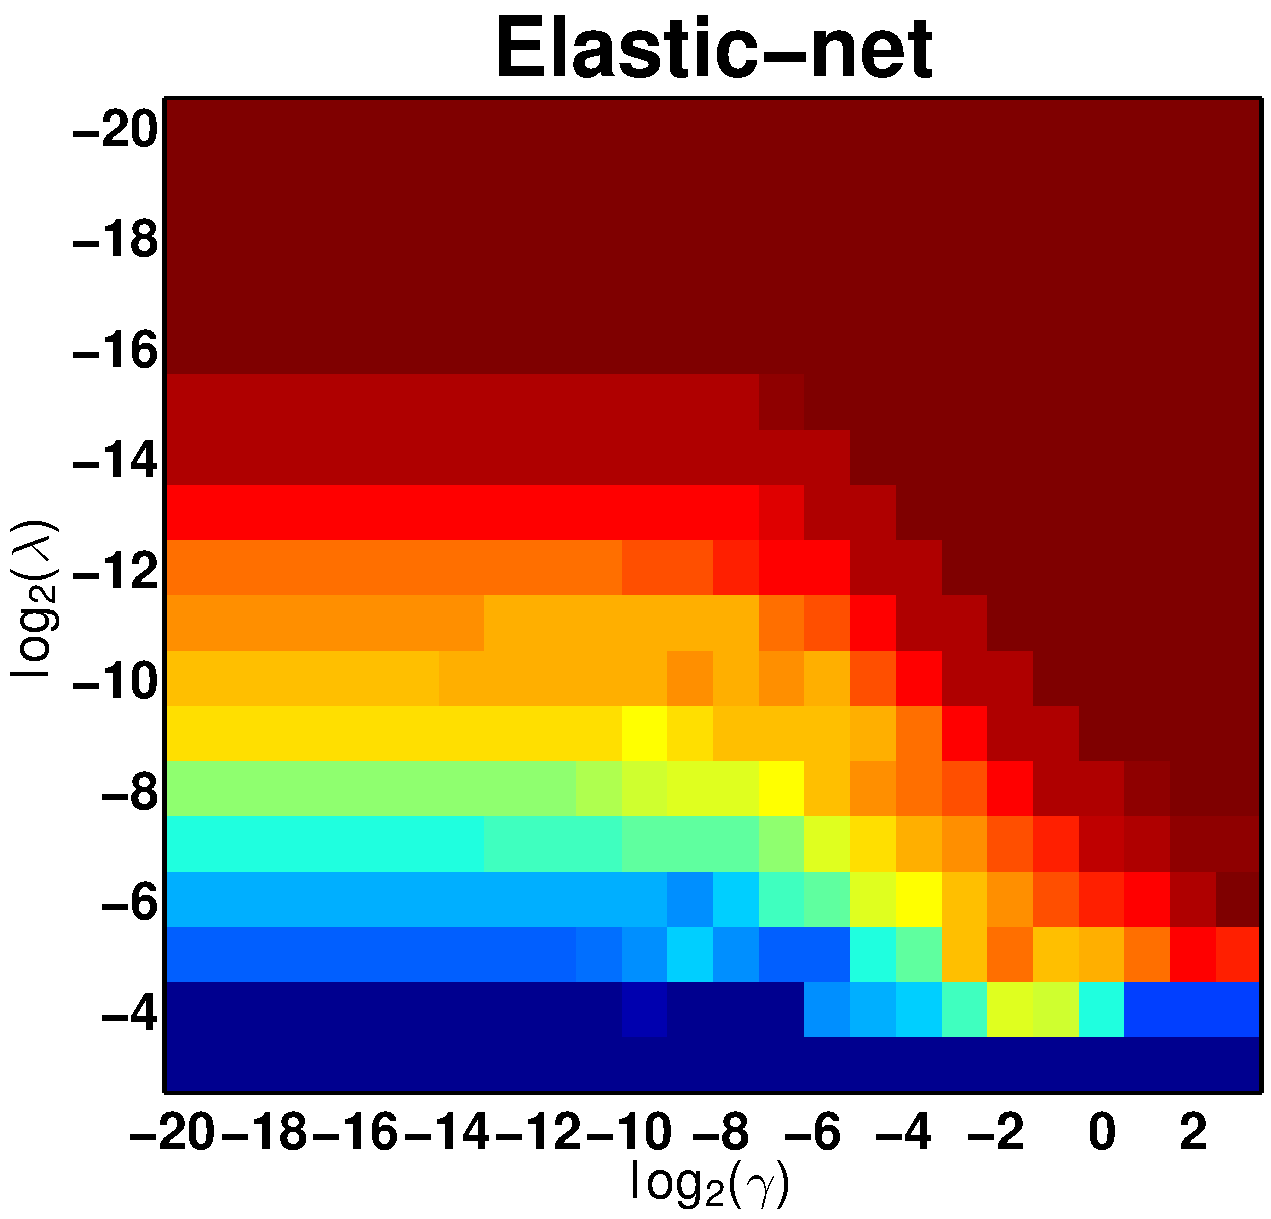
\includegraphics[width=\imwidth,height=\imheight]{exp_gridsearch_acc_enet.pdf} &
	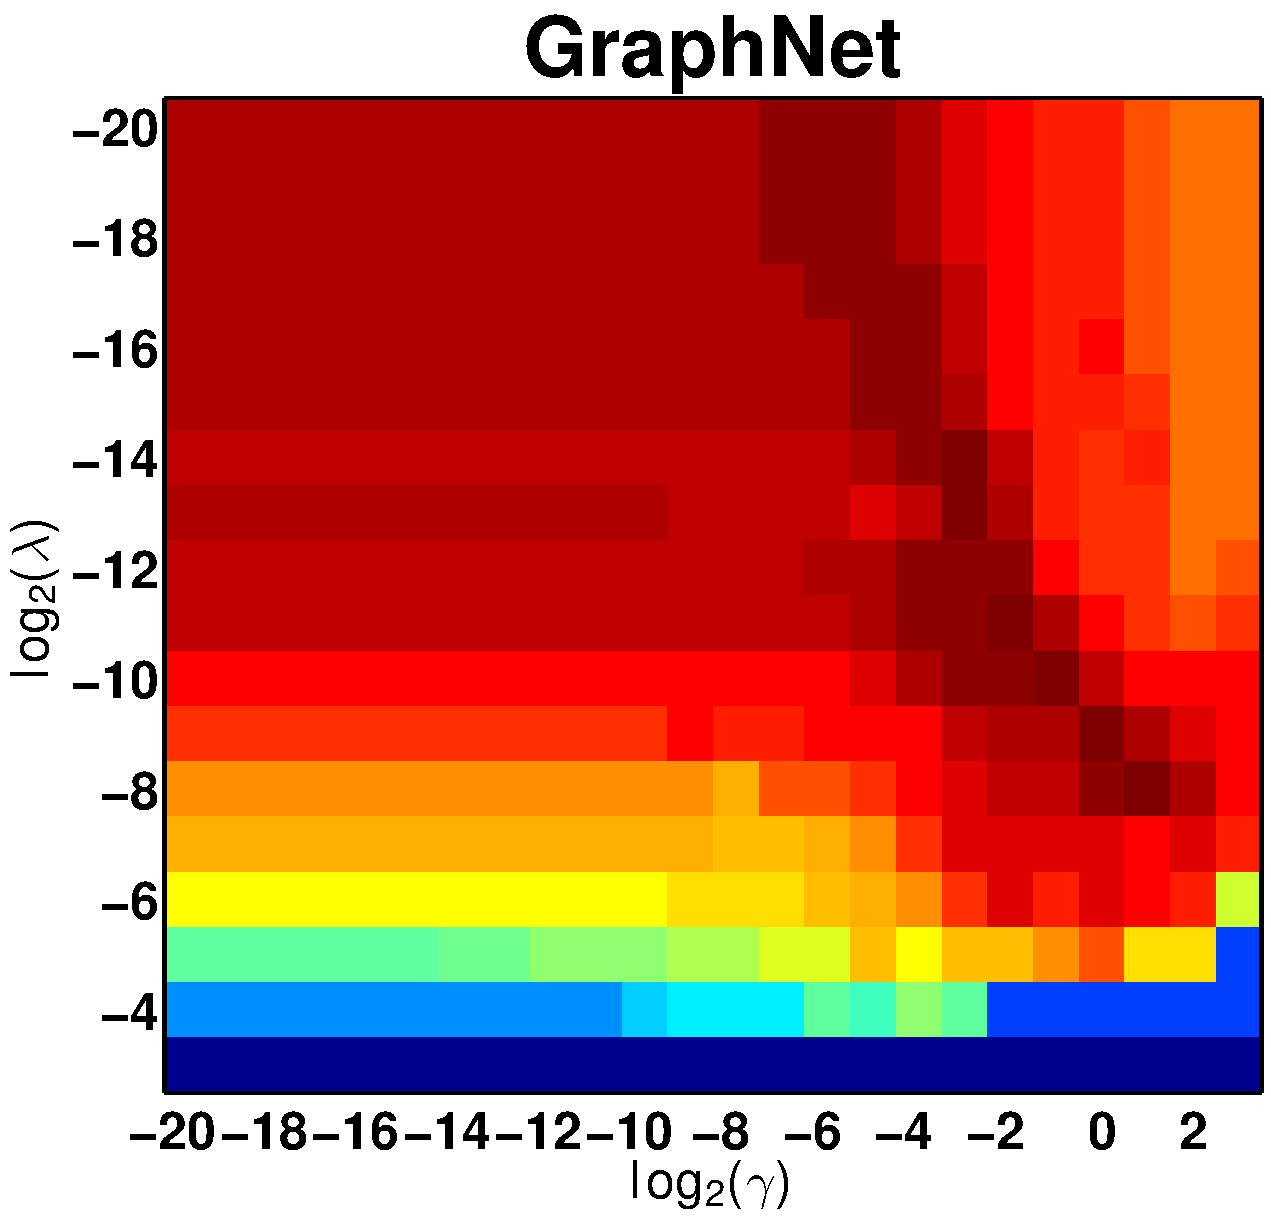
\includegraphics[width=\imwidth,height=\imheight]{exp_gridsearch_acc_gnet.pdf} &
	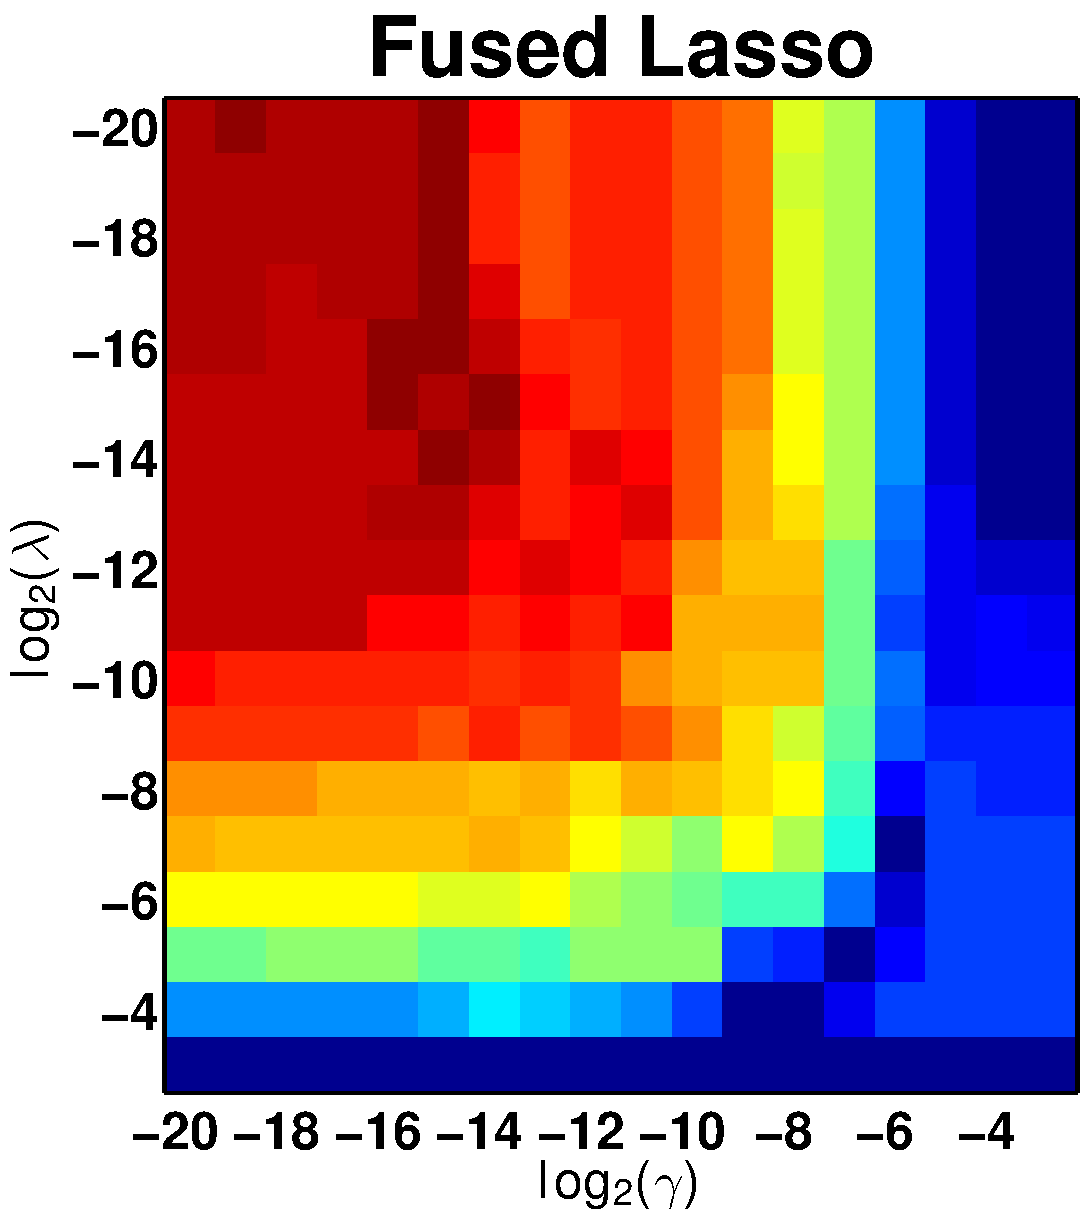
\includegraphics[width=\imwidth,height=\imheight]{exp_gridsearch_acc_flas.pdf} &
	\raisebox{0.02725\linewidth}{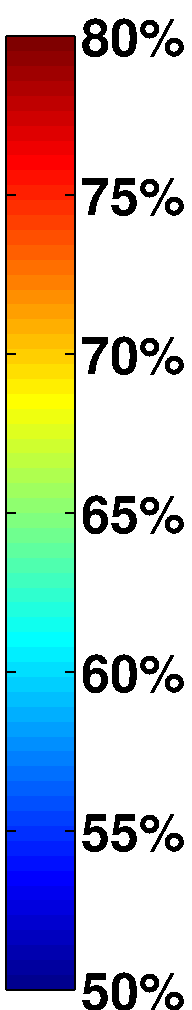
\includegraphics[height=0.268\linewidth]{exp_gridsearch_acc_cbar.pdf}} \vspace{9pt}\\
	\multicolumn{4}{c}{{\textbf{\large{Mean sparsity level (number of features)}}}} \vspace{0pt}\\
	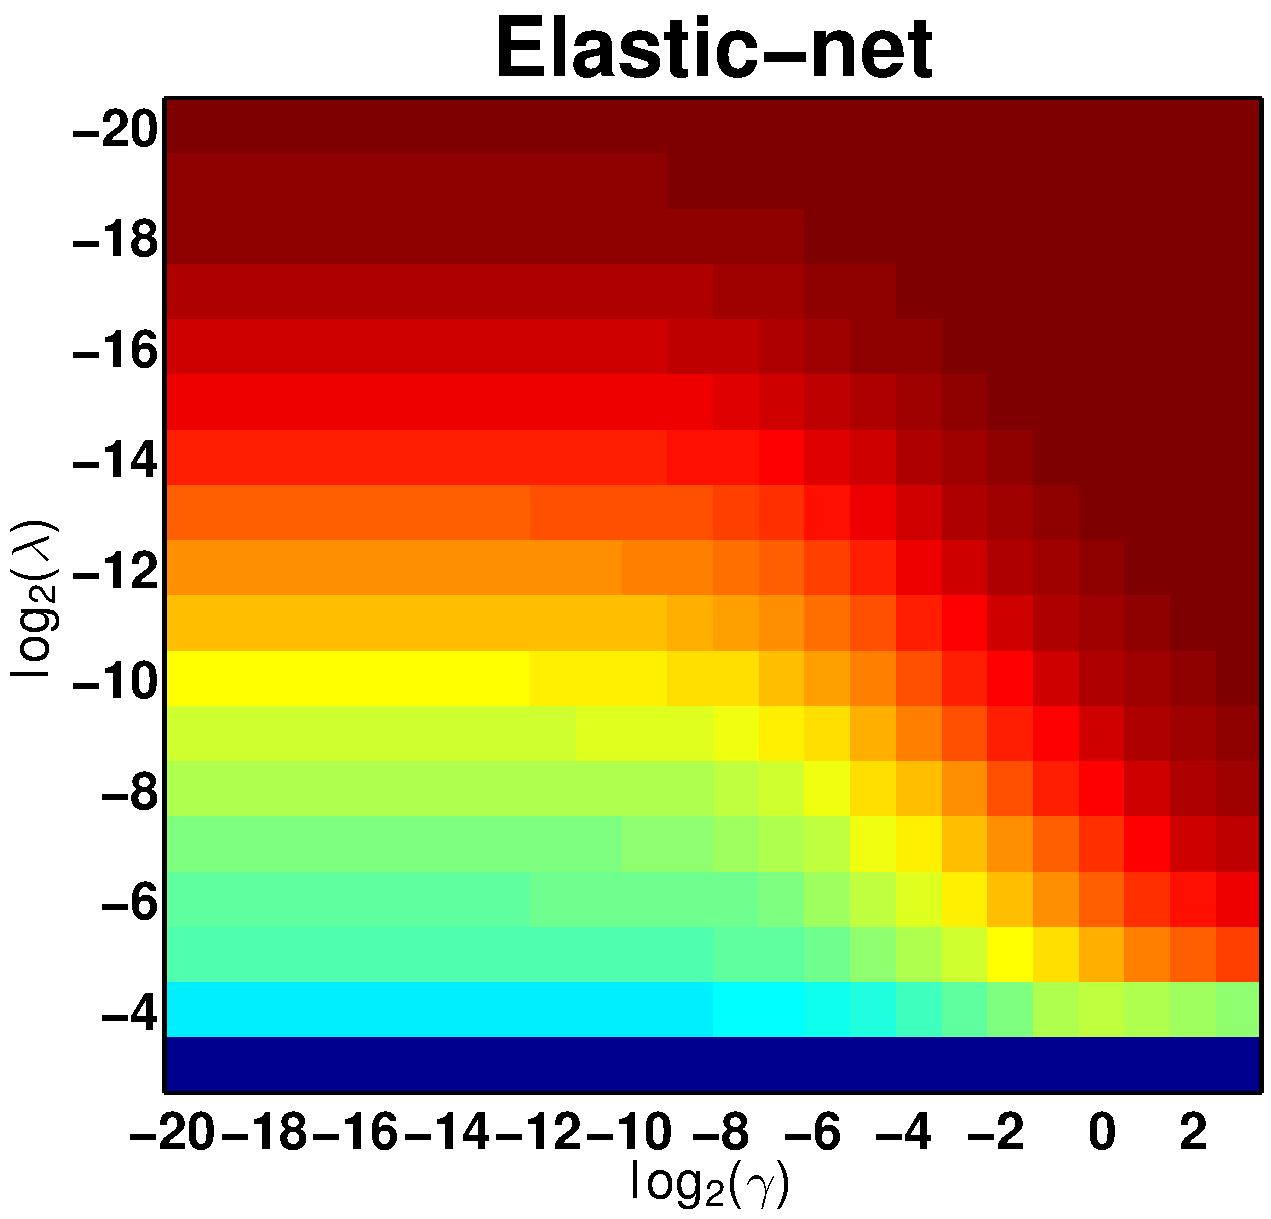
\includegraphics[width=\imwidth,height=\imheight]{exp_gridsearch_nnz_log10_enet.pdf} &
	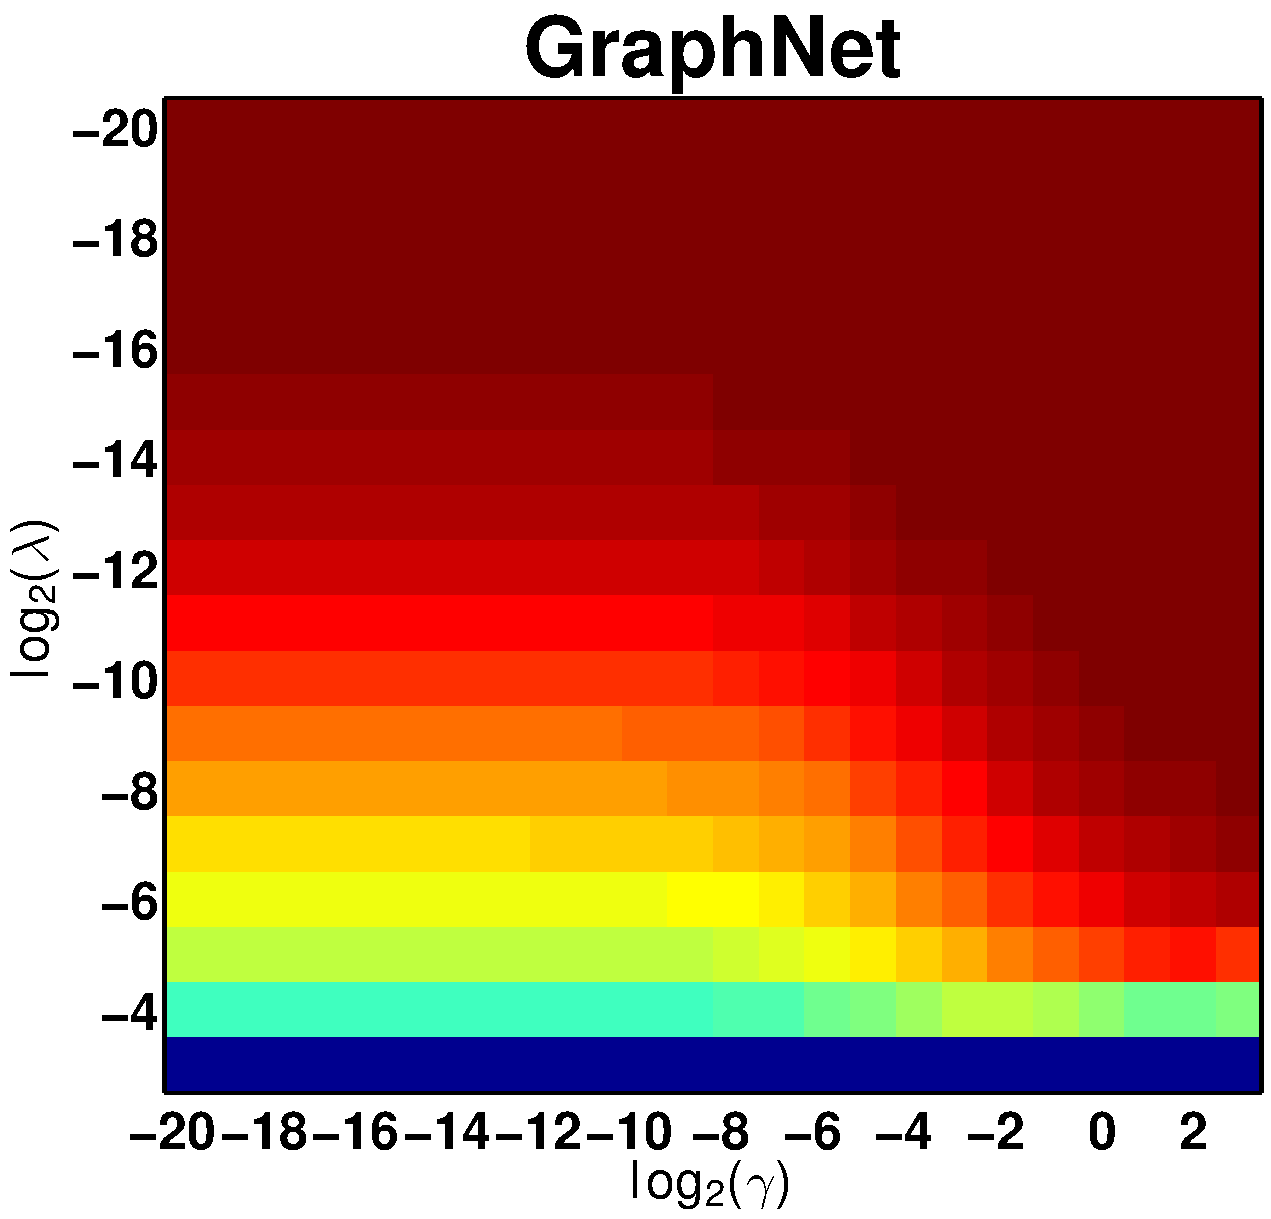
\includegraphics[width=\imwidth,height=\imheight]{exp_gridsearch_nnz_log10_gnet.pdf} &
	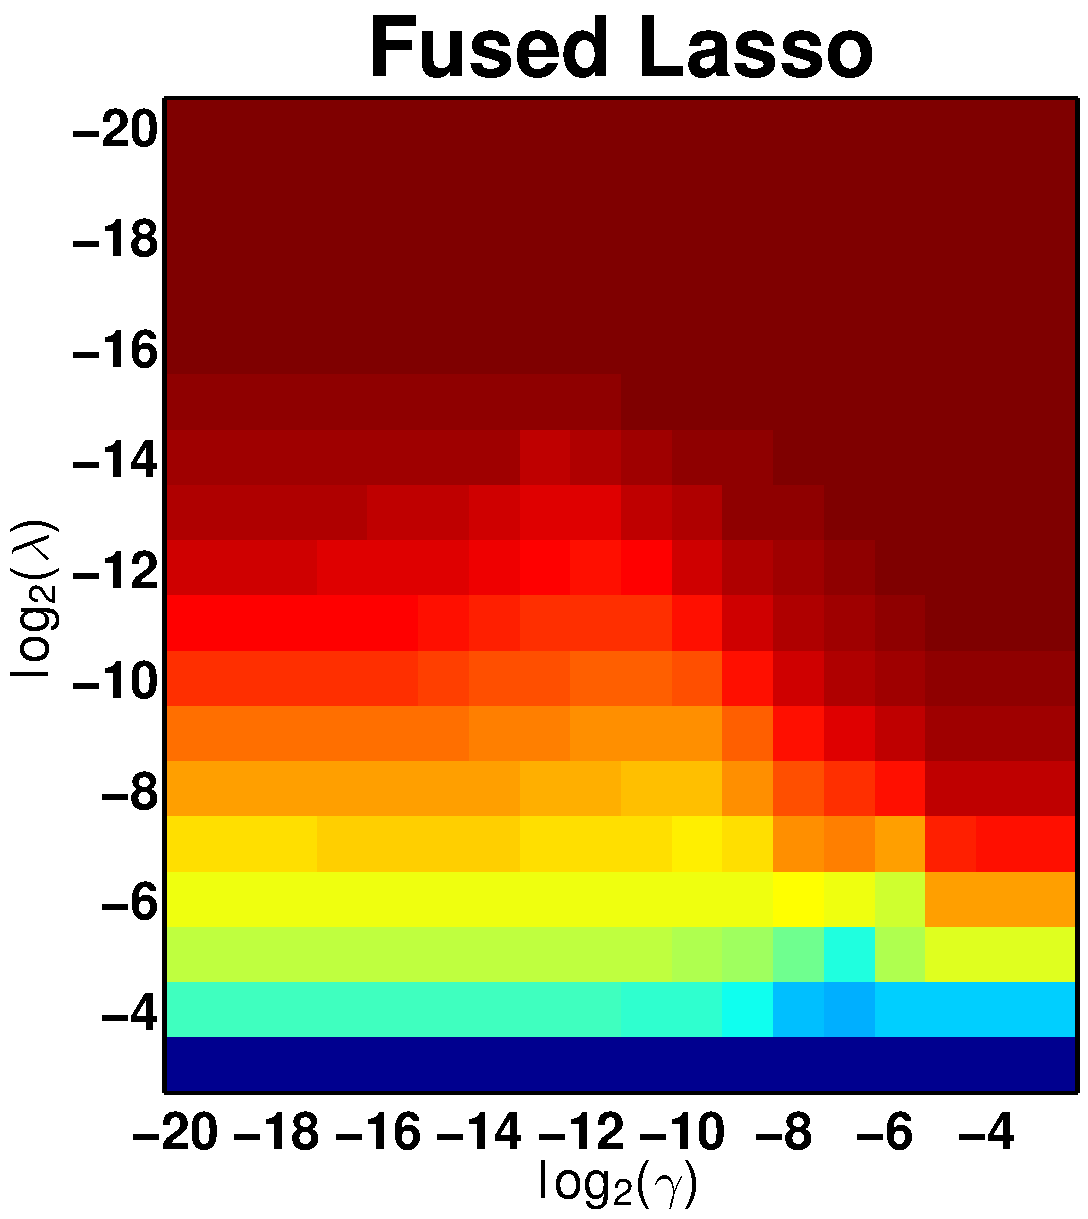
\includegraphics[width=\imwidth,height=\imheight]{exp_gridsearch_nnz_log10_flas.pdf} &
	\hspace{-4pt}\raisebox{0.03225\linewidth}{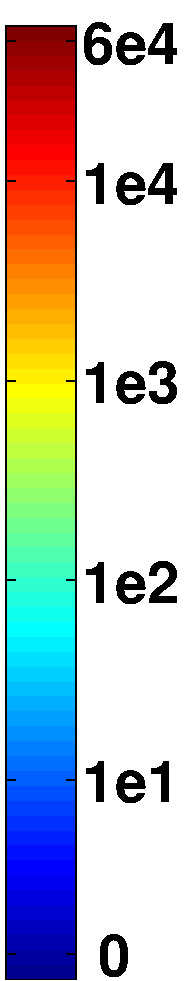
\includegraphics[height=0.26\linewidth]{exp_gridsearch_nnz_cbar_log10.pdf}}\\
%-------------------------------------------------------------------------------------------%
	\addhspace{{(a) Elastic-net}} & \addhspace{{(b) GraphNet}} & \addhspace{{(c) Fused Lasso}} & \vspace{-4pt}	\\
	\end{tabular} 
	\caption{
		Grid search result for the real resting state data (best viewed in color).
		\textbf{Top row}: the classification accuracy evaluated from 10-fold cross-validation.
		\textbf{Bottom row}: the average number of features selected across the cross-validation folds.
		The $(x,y)$-axis corresponds to the two regularization parameters $\lambda$ and $\gamma$.
	}
	\label{fig:grid,search}
\end{figure}
%=================================================================== 

A common practice for choosing the final set of regularization parameters is to select the choice that gives the highest prediction accuracy.
Based on the grid search result reported in Fig.~\ref{fig:grid,search}, one may be tempted to conclude that the prediction models from GraphNet and fused Lasso are not any better than Elastic-net.
However, the ultimate goal in our application is the discovery and validation of connectivity-based biomarkers, thus classification accuracy by itself is not sufficient.
It is equally important for the prediction model to be interpretable  (\eg, sparse) and inform us about the predictive regions residing in the high dimensional connectome space.
From the grid search, we found that for all three regularization methods, the classifiers achieved a good balance between accuracy and sparsity when approximately $3,000$ features ($\approx 5\%$) were selected out of $p=60,031$.
More specifically, Elastic-net, GraphNet, and fused Lasso achieved classification accuracies of $73.5\%$, $70.3\%$, and $71.9\%$, using an average of $3076$, $3403$, and $3140$ features across the cross-validation folds.
Corresponding regularization parameter values $\{\lambda,\gamma\}$ were: $\{2^{-6},2^{-1}\}$, $\{2^{-5},2^{-2}\}$, and $\{2^{-9},2^{-10}\}$.
Therefore, we further analyzed the classifiers obtained from these regularization parameter values. 

During cross-validation, we learned a different weight vector for each partitioning of the dataset.
In order to obtain a single representative weight vector, we took the approach of \cite{Grosenick:2013}, computing the elementwise median of the weight vectors across the cross-validation folds.
Note that this approach possesses attractive theoretical properties; see \cite{Grosenick:2013} and \cite{Minsker:2013} for a detailed discussion.
For visualization and interpretation, we grouped the indices of these weight vectors according to the network parcellation scheme proposed by \cite{Yeo:2011}, and augmented this parcellation with subcortical regions and cerebellum derived from the parcellation of \cite{AAL:2002} (see Table~\ref{table:network}); these weight vectors are then reshaped them into $347\times 347$ symmetric matrices with zeroes on the diagonal.
Furthermore, we generated trinary representations of these matrices in order to highlight their support structures, where red, blue, and white denotes positive, negative, and zero entries respectively.
The resulting matrices are displayed in Fig.~\ref{fig:exp,median}.

%%%%%%%%%%%%%%%% Experiment Result Figures %%%%%%%%%%%%%%%%%%%%%%%%%%
%*************************************************************************%
% - script looks unholy, but this ensures a table and figure to be displayed together on top of the page
% - http://tex.stackexchange.com/questions/47900/place-a-minipage-on-the-top-of-a-page
% - http://tex.stackexchange.com/questions/55337/how-to-use-figure-inside-a-minipage
\begin{figure}[t!]\begin{minipage}{\textwidth}
	\renewcommand{\imwidth}  {0.3\linewidth}
	\setlength{\tabcolsep}{1pt} 
	\begin{tabular}{cccc}
	\multicolumn{4}{c}{{\textbf{\large{Median Weight Vector}}}} \vspace{0pt} \\
	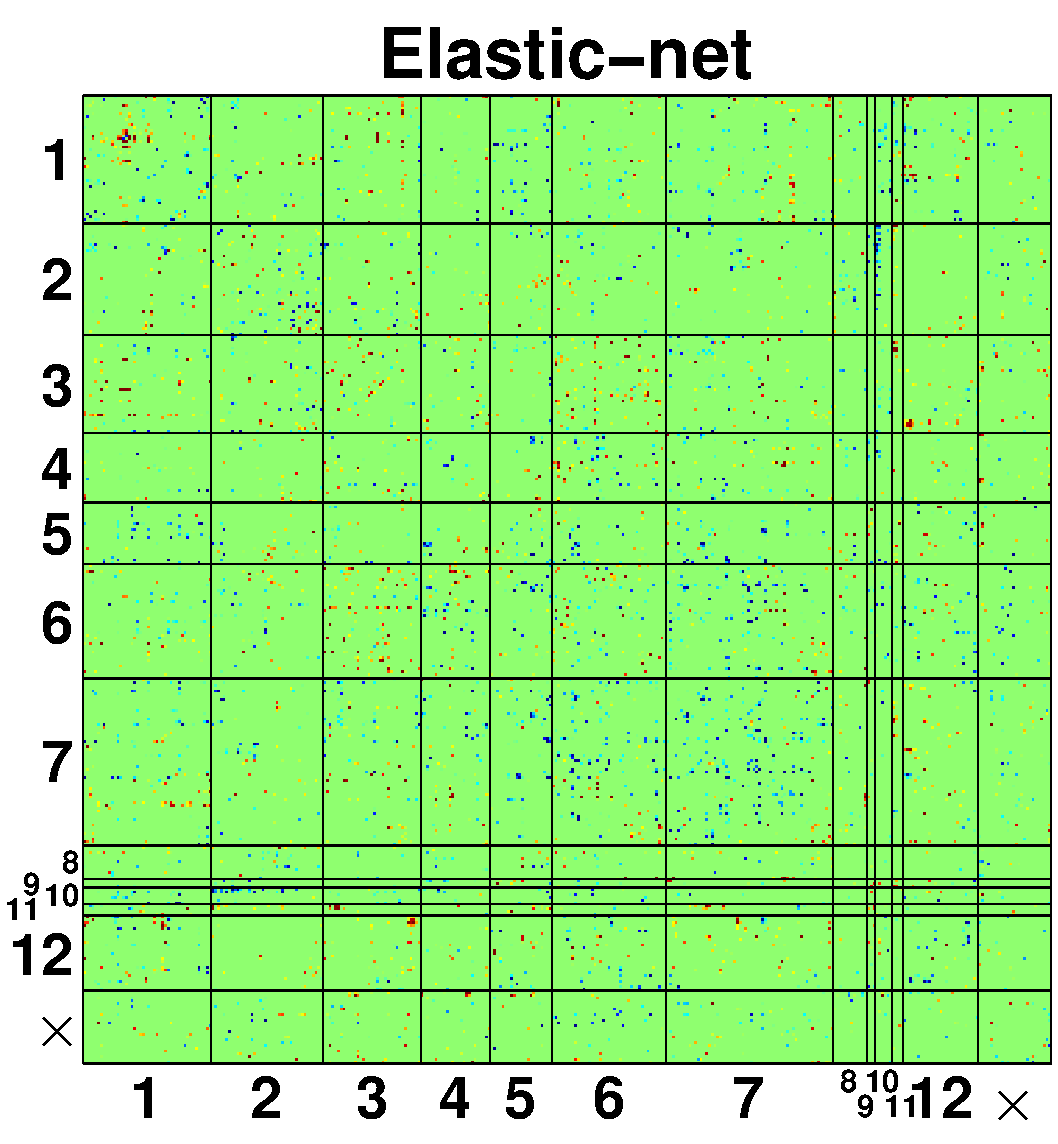
\includegraphics[width=\imwidth]{exp_median_wmat_enet.pdf} &
	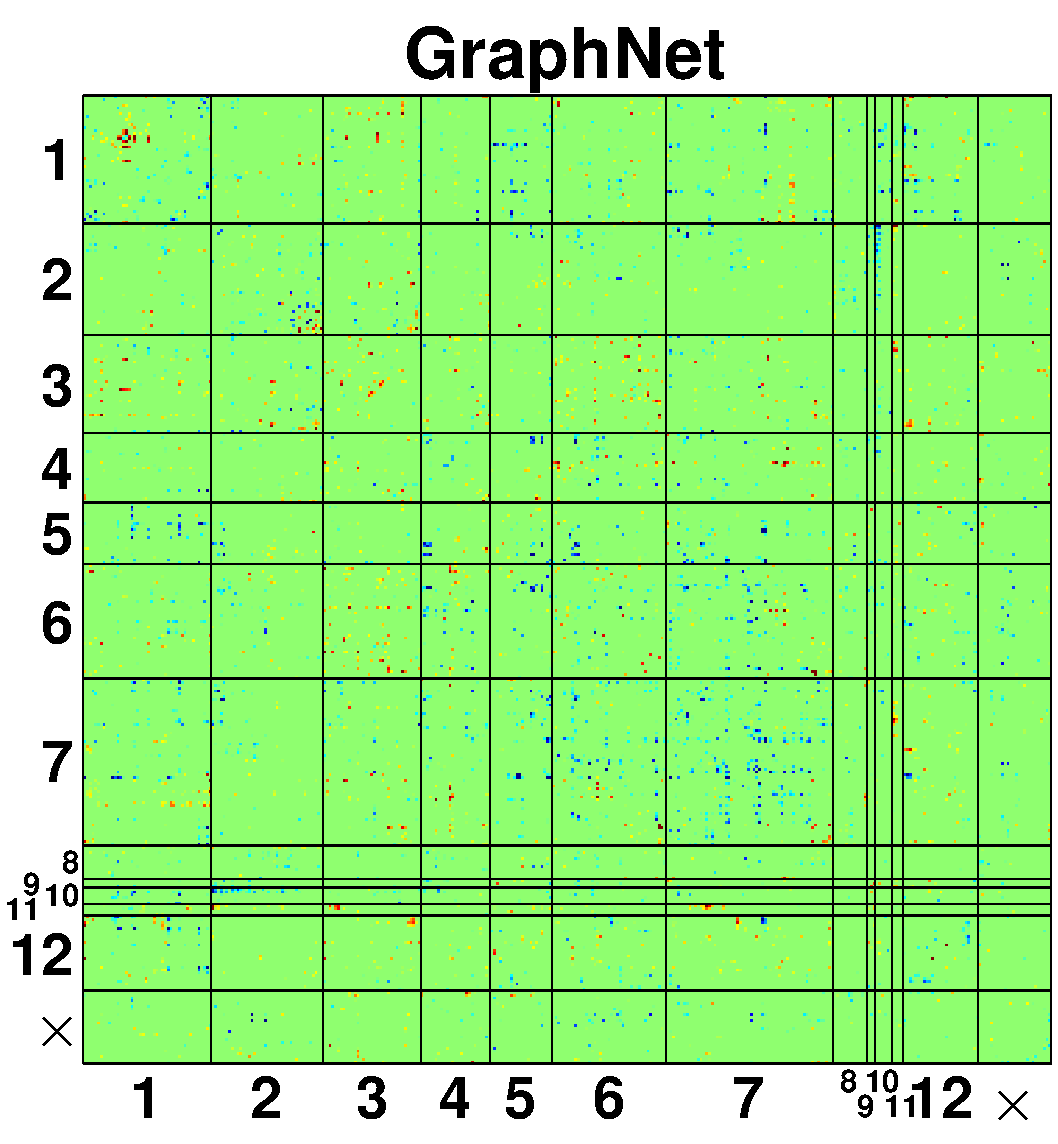
\includegraphics[width=\imwidth]{exp_median_wmat_gnet.pdf} &
	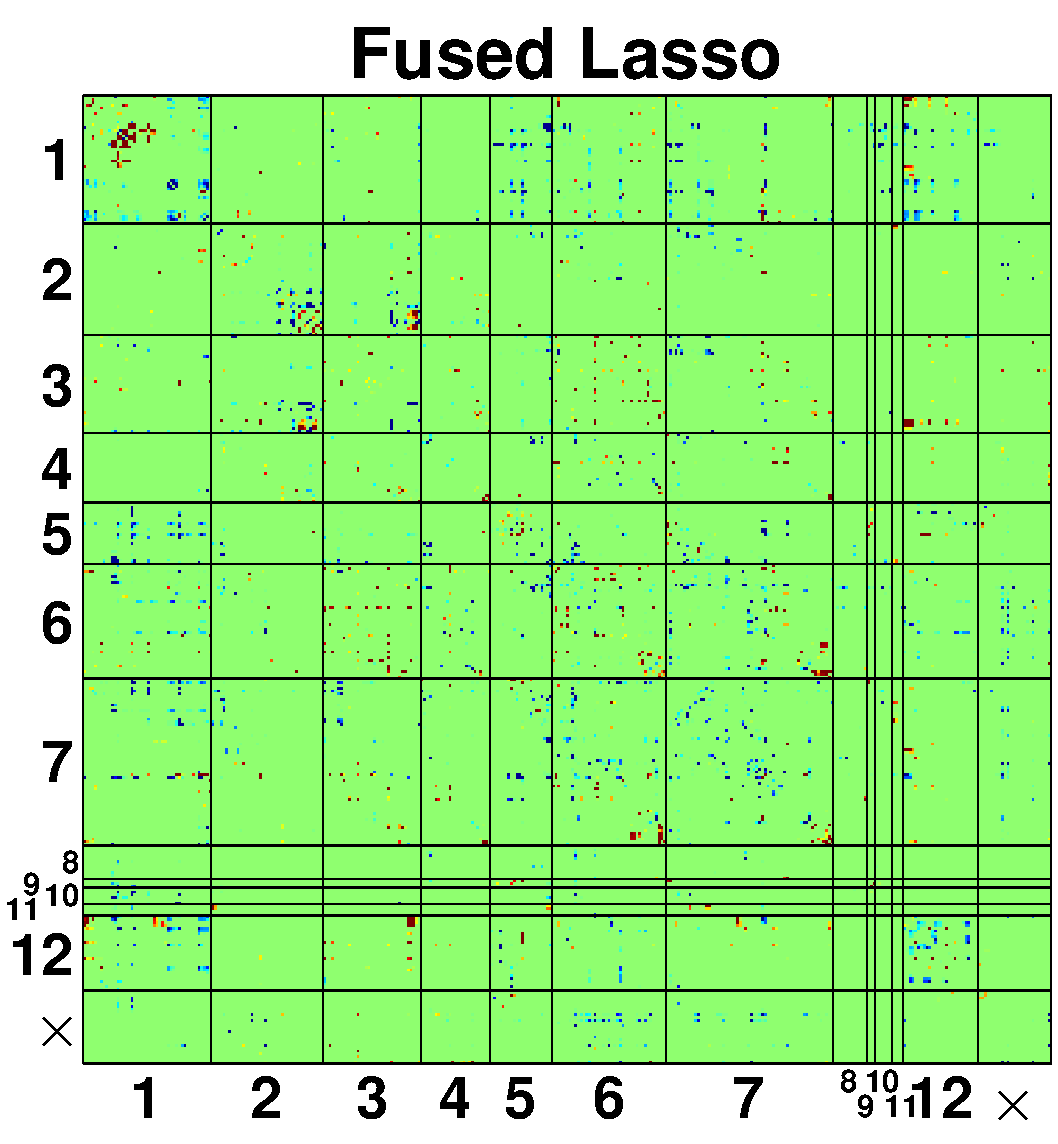
\includegraphics[width=\imwidth]{exp_median_wmat_flas.pdf} &
	\raisebox{0.02225\linewidth}{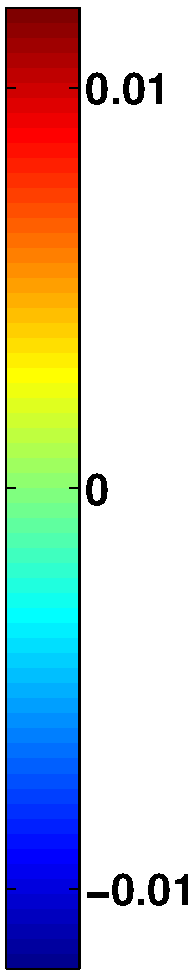
\includegraphics[height=0.27675\linewidth]{exp_median_wmat_cbar.pdf}} \vspace{4pt}\\
	\multicolumn{4}{c}{{\textbf{\large{Median Weight Vector Support}}}} \vspace{0pt} \\
	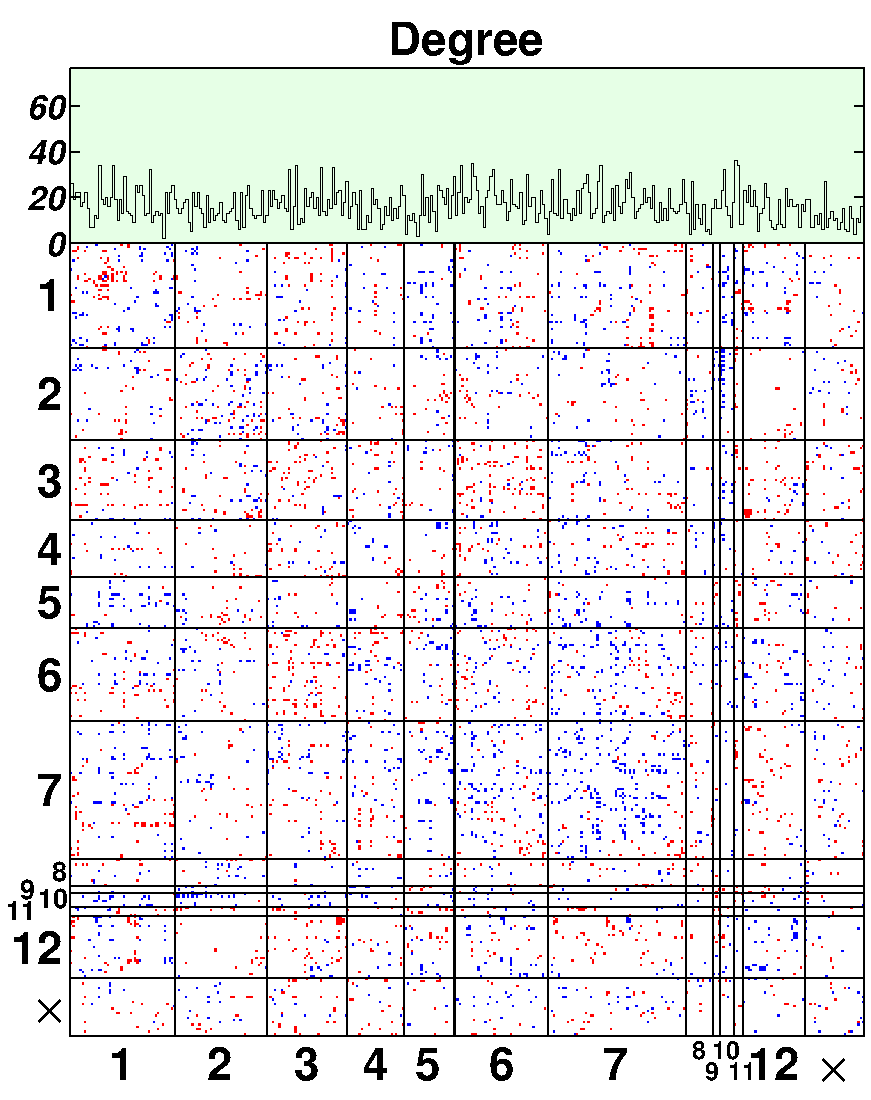
\includegraphics[width=\imwidth]{exp_median_supp_enet.pdf} &
	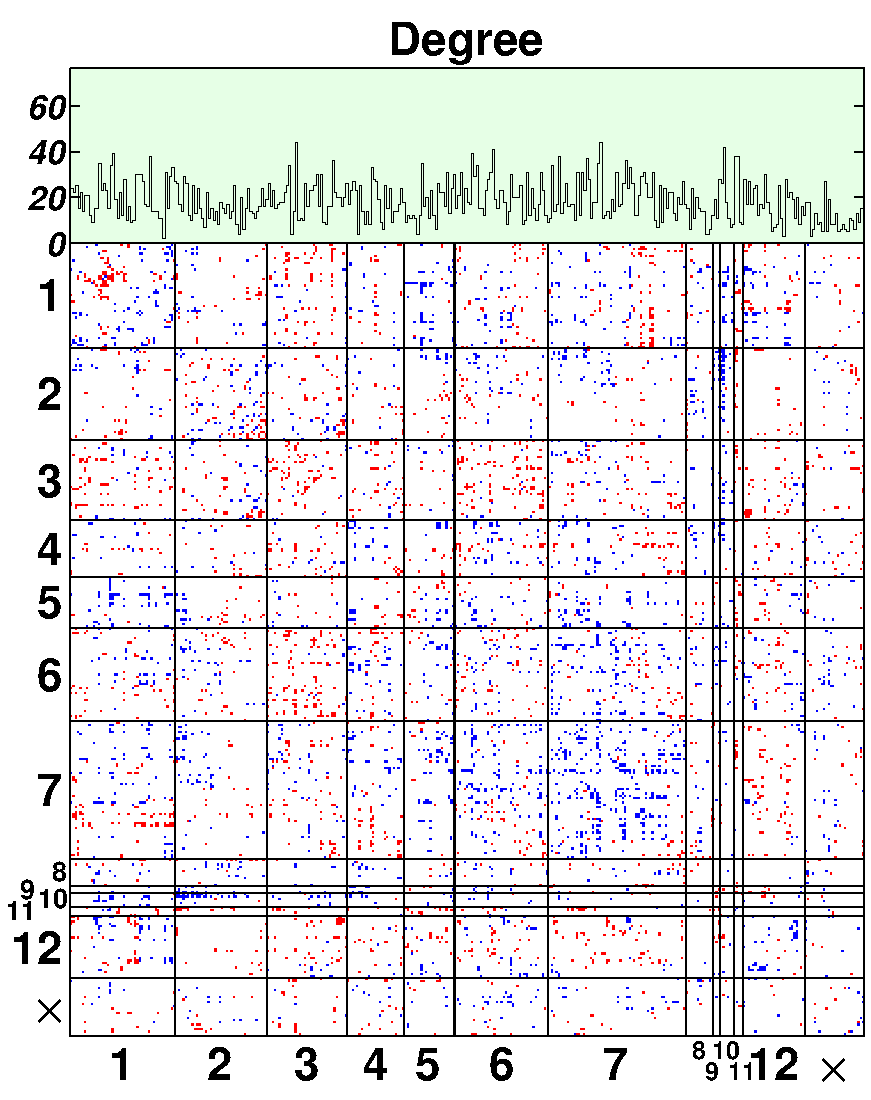
\includegraphics[width=\imwidth]{exp_median_supp_gnet.pdf} &
	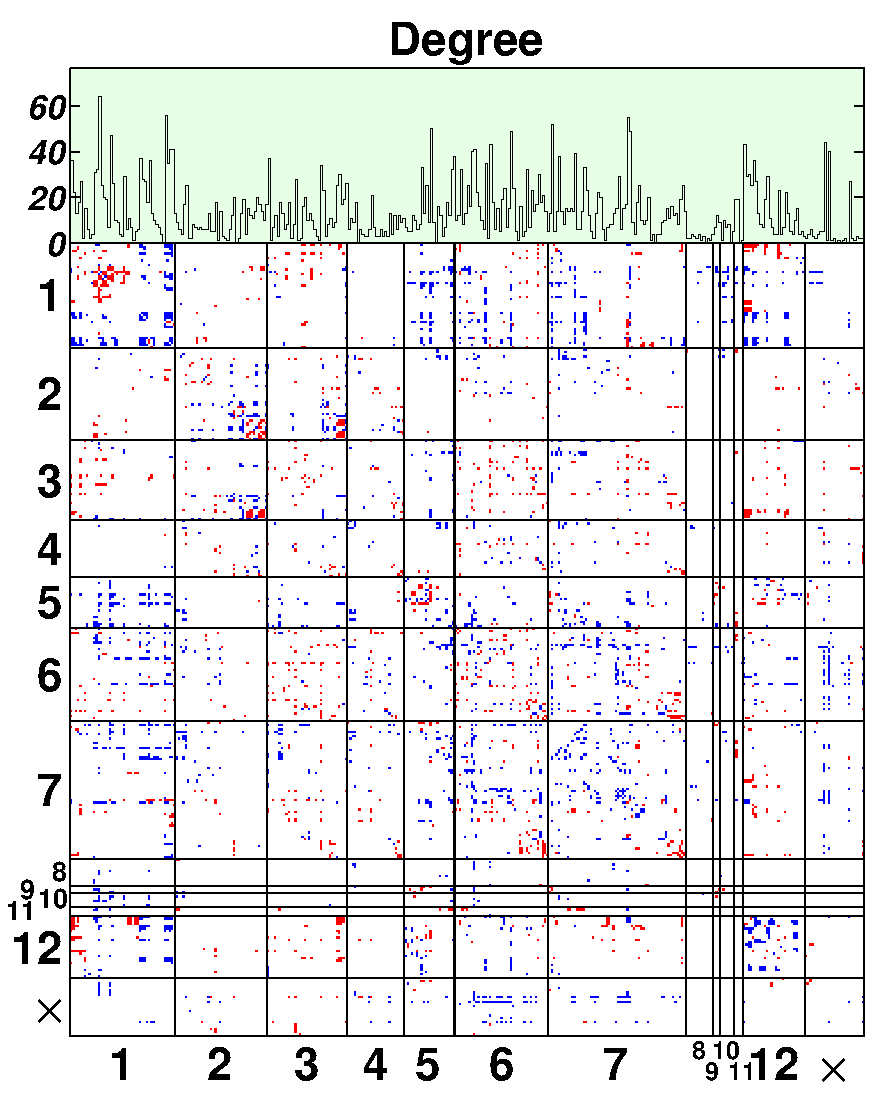
\includegraphics[width=\imwidth]{exp_median_supp_flas.pdf} &
	\hspace{-2pt}\raisebox{0.0215\linewidth}{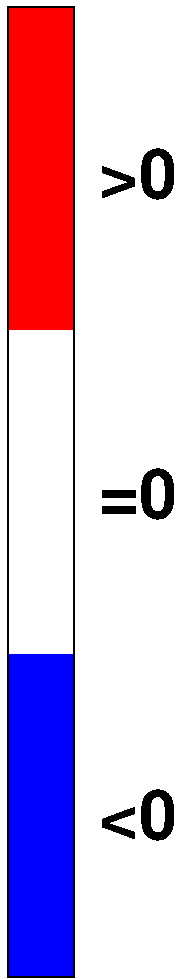
\includegraphics[height=0.2755\linewidth]{exp_median_supp_cbar.pdf}} \vspace{-2pt} \\
\addhspace{{(a) Elastic-net}} & \addhspace{{(b) GraphNet}} & \addhspace{{(c) Fused Lasso}} & \vspace{-5pt}	\\
	\end{tabular} 
	\captionof{figure}{
	Weight vectors (reshaped into symmetric matrices) generated by computing the elementwise median of the estimated weight vectors across the cross-validation folds (best viewed in color).  
	The rows and columns of these matrices are grouped according to the network parcellation scheme proposed by \cite{Yeo:2011}, which is reported in Table~\ref{table:network}.
	The top row displays the heatmap of the estimated weight vectors, whereas the bottom row displays their support structures, with red, blue, and white indicating positive, negative, and zero entries respectively.
	In order to highlight the structure of the estimated weight vectors, the bottom row further plots the degree of the nodes, \ie, the number of connections a node makes with the rest of the network.
	}
	\label{fig:exp,median}
	\vspace{12pt}
%=============== yeo table ================================= 
	\centering
	\setlength{\tabcolsep}{8pt} 
	\begin{tabular}{llll}
		\hline
		\multicolumn{4}{c}{Network Membership Table ($\times$ is ``unlabeled'')}  \\ 
		\hline\hline
		 1. Visual		& 2. Somatomotor 	 & 3. Dorsal Attention 	& 4. Ventral Attention \\
		 5. Limbic 		& 6. Frontoparietal  & 7. Default	 		& 8. Striatum 		\\
		 9. Amygdala 		& 10. Hippocampus	 & 11. Thalamus		& 12. Cerebellum \\
		\hline
	\end{tabular}\vspace{-4pt}
	\captionof{table}{Network parcellation of the brain proposed by \cite{Yeo:2011}.  In our real resting state fMRI study, the indices of the estimated weight vectors are grouped according to this parcellation scheme; see Fig.~\ref{fig:exp,median}.}
	\label{table:network}
	\vspace{-8pt}
\end{minipage}\end{figure}
%%%%%%%%%%%%%%%%%%%%%%%%%%%%%%%%%%%%%%%%%%%%%%%%%%%%%%%%%%%%%%%%%%%%%

From these figures, one can observe that Elastic-net yields solutions that are scattered throughout the connectome space, which can be problematic for interpretation.
In contrast, the weight vector returned from GraphNet has a much smoother structure, demonstrating the impact of the smooth spatial penalty; this is arguably a far more sensible structure from a biological standpoint.
Finally, the weight vector from fused Lasso reveals systematic sparsity patterns with multiple contiguous clusters present, indicating that the predictive regions are compactly localized in the connectome space (\eg, see the rich connectivity patterns present in the intra-visual and intra-cerebellum network).
It is noteworthy the fused Lasso not only appears to identify more densely packed patches of abnormalities in certain regions, it also generates large areas of relative sparsity (\eg, see somatomotor network interconnections with other networks, and the nodes that fall outside the augmented Yeo parcellation scheme, which are labeled~``$\times$''). 
These areas are more sparse in the fused Lasso map, and this appears to be consistent with existing knowledge of connectivity alterations in schizophrenia (see Sec.~\ref{subsec:disc,real,data} of the Discussion). 
In addition, the weight vector estimate from fused Lasso appears to implicate certain nodes more often in connectivity alterations. 
In order to emphasize this point, the bottom row in Fig.~\ref{fig:exp,median} also plots the degree of the nodes, \ie, the number of connections a node makes with the rest of the nodes (this is another example of ``spatial contiguity'' in the $6$-D connectome space).

Finally, in order to convey the regional distribution of the edges recovered by fused Lasso, we rendered implicated edges on canonical $3$-D brains (Fig.~\ref{fig:bnv,median}; these figures were generated with the BrainNet Viewer, \url{http://www.nitrc.org/projects/bnv/}).
We focus on the three sets of network-to-network connections, intra-frontoparietal, frontoparietal-default, and intra-cerebellum, as these three networks have particularly extensive evidence of their involvement in schizophrenia (see Discussion in Sec.~\ref{sec:discussion}).
It is noteworthy that lateral prefrontal cortex, an important region in frontoparietal network, is well represented in the fused Lasso map. 
Edges involving this region represent $39.3\%$ of the intra-frontoparietal connections and $43.6\%$ of the frontoparietal-default network connections. 
This finding is consistent with previous studies of schizophrenia that emphasize the importance of this region (see Discussion in Sec.~\ref{sec:discussion}). 

%%%%%%%%%% brain net viewer fig %%%%%%%%%%%%%%%%%%%%
\renewcommand{\imheight}  {0.3\textwidth}
\renewcommand{\VSPACE}{\vspace{12pt}}
\renewcommand{\VSPACEE}{\vspace{0pt}}
% http://stackoverflow.com/questions/1963923/adding-full-page-figures-in-latex-how
\begin{figure}[ptbh]
	\centering	
	\setlength{\tabcolsep}{8pt}
	\myfbox{\begin{tabular}{cc}
		\vspace{-8pt}\\
		
\includegraphics[width=0.225\textwidth]{YeoKey.png} & \hspace{10pt}
		\raisebox{7pt}{
\includegraphics[width=0.4\textwidth]{schiz_edge_legend.png}}  \vspace{0pt}\\
		\textbf{(node color)} & \textbf{(edge color)} \vspace{-2pt} \\ 
	\end{tabular}}\vspace{11pt} \\
	\begin{tabular}{ccc}
		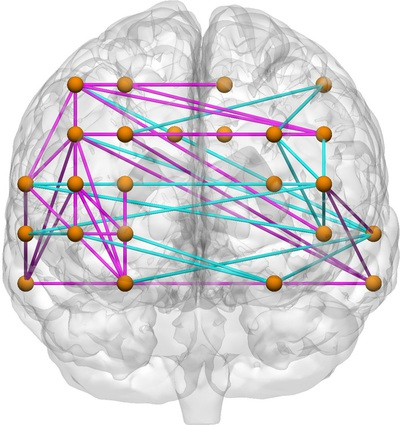
\includegraphics[height=\imheight]{6-6_anterior_flas.jpg}  &
		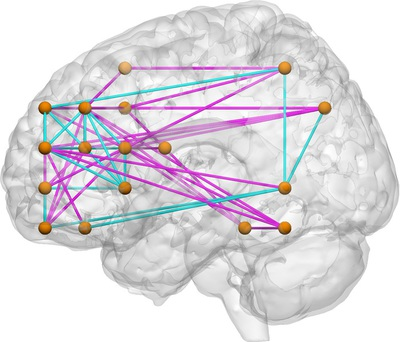
\includegraphics[height=\imheight]{6-6_lateral_flas.jpg}  &
		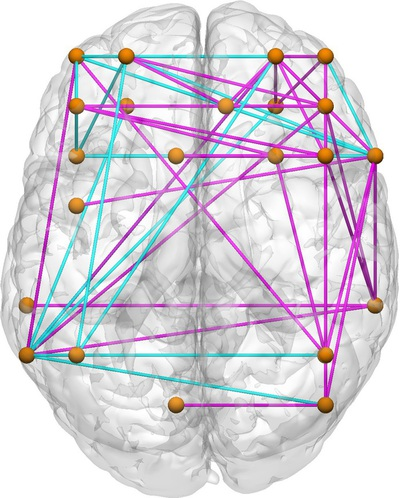
\includegraphics[height=\imheight]{6-6_superior_flas.jpg} \VSPACEE\\
		\multicolumn{3}{c}{\textbf{\large{Intra-Frontoparietal (6-6)}}} \VSPACE \\
		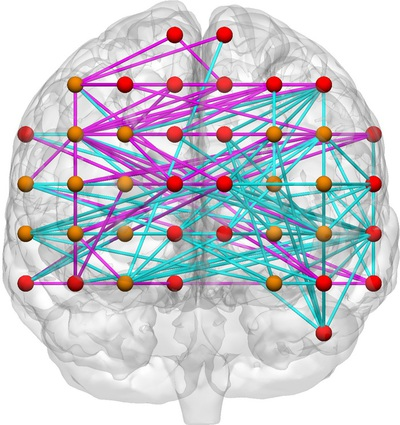
\includegraphics[height=\imheight]{6-7_anterior_flas.jpg}  &
		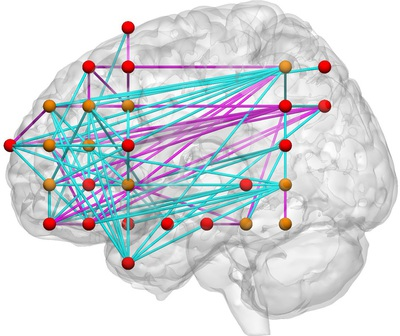
\includegraphics[height=\imheight]{6-7_lateral_flas.jpg}  &
		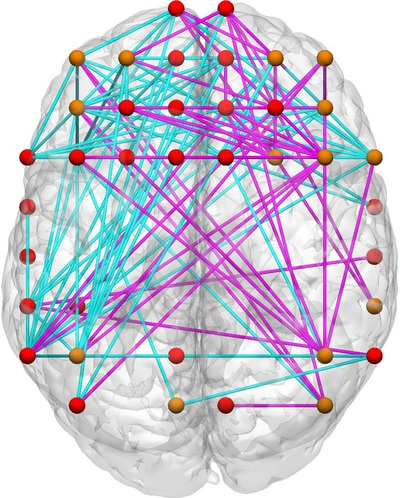
\includegraphics[height=\imheight]{6-7_superior_flas.jpg} \VSPACEE\\
		\multicolumn{3}{c}{\textbf{\large{Frontoparietal-Default (6-7)}}} \VSPACE \\
		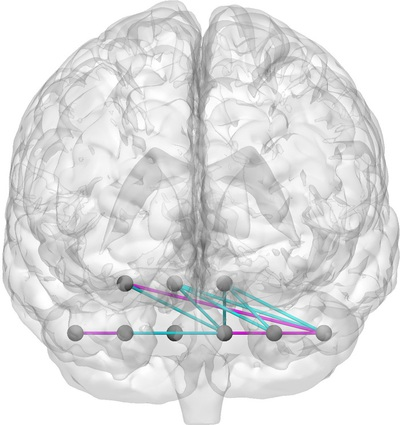
\includegraphics[height=\imheight]{12-12_anterior_flas.jpg}  &
		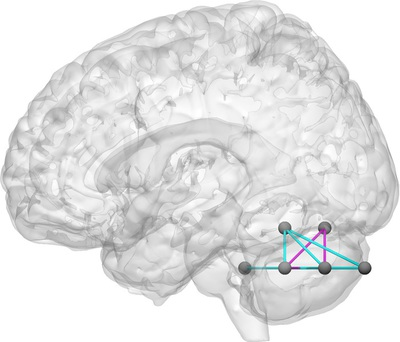
\includegraphics[height=\imheight]{12-12_lateral_flas.jpg}  &
		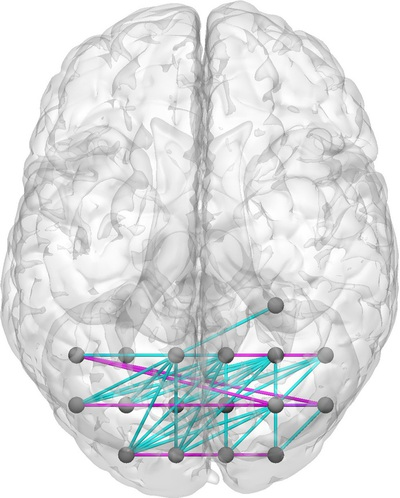
\includegraphics[height=\imheight]{12-12_superior_flas.jpg} \VSPACEE\\
		\multicolumn{3}{c}{\textbf{\large{Intra-Cerebellum (12-12)}}}  \\
	\end{tabular}
	\caption{
	Nonzero edge values of the median weight vector generated from the fused Lasso regularized SVM.  
	For three sets of network-to-network connections, we rendered abnormal connections separately on anterior, sagittal, and axial views of a canonical brain. 
	Notice the prominent involvement of lateral prefrontal regions in connections within frontoparietal network and in connections between frontoparietal network and default network.
	}
	\label{fig:bnv,median}
\end{figure}
%%%%%%%%%%%%%%%%%%%%%%%%%%%%%%%%%%%%%%%%%%%%%%%%%

%===================================================================%
%		 		Computational consideration
%===================================================================%
\subsection{Computational considerations}
It is important to note that the benefit of spatial regularization comes with higher computational expense.
To illustrate this point, we ran the ADMM algorithms for Elastic-net, GraphNet, and fused Lasso for $1000$ iterations on the full resting state dataset using regularization parameter values $\{\lambda,\gamma\}=\{2^{-15},2^{-15}\}$ and compared their computation times
(the algorithm for Elastic-net is reported in \ref{appendix,admm,enet}, whereas the algorithms for GraphNet and fused Lasso are reported in Algorithm~\ref{alg:admm}).
This timing experiment was implemented in MATLAB version $7.13.0$ on a desktop PC with Intel quad-core $3.40$ GHz CPU and $12$ GB RAM.
The total computation times for Elastic-net, GraphNet, and fused Lasso were $17.04$ seconds, $96.07$ seconds, and $112.45$ seconds respectively.
The increase in computation time for GraphNet and fused Lasso stems from the fact that unlike the \elltwo-penalty in Elastic-net, the spatial penalty $\norm{\C\w}_q^q,\; {q\in\{1,2\}}$ is not separable across the coordinates of \w.
To address this difficulty, the variable splitting strategy proposed for GraphNet and fused Lasso~\eqref{eqn:admm,splitting2} contains four constraint variables, which is two more than the splitting proposed for Elastic-net~\eqref{eqn:splitting,enet}; as a consequence, the ADMM algorithms for GraphNet and fused Lasso contain two additional subproblems.
Furthermore, the computational bottlenecks of the ADMM algorithms for GraphNet and fused Lasso are the $6$-D FFT and inverse-FFT operations~\eqref{eqn:v4,fft}, which are not conducted for the Elastic-net.
Therefore, if achieving high classification accuracy is the central goal, then Elastic-net would be the most sensible and practical choice, as it yields good classification accuracy and is by far the fastest among the three regularization methods we studied.

%% new segment: battle between our fused Lasso and G. Ye's fused Lasso SVM
Finally, in order to assess the practical utility of our proposed algorithm with respect to existing methods, we conducted another timing experiment using the ADMM algorithm proposed by \cite{Gui-Bo-Ye:2011}, which also solves fused Lasso regularized SVM.
It is important to note that the variable splitting scheme they employ is different from the one we introduce, and consequently, their method requires the following matrix inversion problem to be solved for one of the ADMM updates:
\begin{equation}
\w\iterp \leftarrow 
	\left(
		\X^T\X + \C^T\C + \BI_p
	\right)\inv  
	\big(
		\X^T\Y^T [\va\iter-\ua\iter] +[\vb\iter-\ub\iter] + \C^T[\vc\iter-\uc\iter]
	\big).
	%\label{eqn:ye,inversion}
	\nonumber
\end{equation}
As suggested in \cite{Gui-Bo-Ye:2011}, we applied the conjugate gradient algorithm to numerically solve this large scale matrix inversion problem\footnote{The conjugate gradient algorithm was ran until either the \elltwo-norm of the residual fell below $1\times 10^{-3}$ or the algorithm reached $60$ iterations.}.
Using the same experimental protocol as our first timing experiment, we ran Ye and Xie's algorithm for $1000$ iterations on the full resting state dataset, which resulted in a total computation time of $331.36$ seconds,
which is nearly three times longer than the algorithm we proposed. 
This illustrates the practical benefit of our proposed variable splitting and data augmentation scheme, which allows all the ADMM updates to be solved analytically.
